\documentclass[
  digital,     %% The `digital` option enables the default options for the
               %% digital version of a document. Replace with `printed`
               %% to enable the default options for the printed version
               %% of a document.
%%  color,       %% Uncomment these lines (by removing the %% at the
%%               %% beginning) to use color in the printed version of your
%%               %% document
  oneside,     %% The `oneside` option enables one-sided typesetting,
               %% which is preferred if you are only going to submit a
               %% digital version of your thesis. Replace with `twoside`
               %% for double-sided typesetting if you are planning to
               %% also print your thesis. For double-sided typesetting,
               %% use at least 120 g/m² paper to prevent show-through.
  nosansbold,  %% The `nosansbold` option prevents the use of the
               %% sans-serif type face for bold text. Replace with
               %% `sansbold` to use sans-serif type face for bold text.
  nocolorbold, %% The `nocolorbold` option disables the usage of the
               %% blue color for bold text, instead using black. Replace
               %% with `colorbold` to use blue for bold text.
  lof,         %% The `lof` option prints the List of Figures. Replace
               %% with `nolof` to hide the List of Figures.
  lot,         %% The `lot` option prints the List of Tables. Replace
               %% with `nolot` to hide the List of Tables.
]{fithesis4}
%% The following section sets up the locales used in the thesis.
\usepackage[resetfonts]{cmap} %% We need to load the T2A font encoding
\usepackage[T1,T2A]{fontenc}  %% to use the Cyrillic fonts with Russian texts.
\usepackage[
  main=english, %% By using `czech` or `slovak` as the main locale
                %% instead of `english`, you can typeset the thesis
                %% in either Czech or Slovak, respectively.
  english, czech, slovak %% The additional keys allow
]{babel}        %% foreign texts to be typeset as follows:
%%
%%   \begin{otherlanguage}{german}  ... \end{otherlanguage}
%%   \begin{otherlanguage}{russian} ... \end{otherlanguage}
%%   \begin{otherlanguage}{czech}   ... \end{otherlanguage}
%%   \begin{otherlanguage}{slovak}  ... \end{otherlanguage}
%%
%% For non-Latin scripts, it may be necessary to load additional
%% fonts:
\usepackage{paratype}
\def\textrussian#1{{\usefont{T2A}{PTSerif-TLF}{m}{rm}#1}}
%%
%% The following section sets up the metadata of the thesis.
\thesissetup{
    date        = \the\year/\the\month/\the\day,
    university  = mu,
    faculty     = fi,
    type        = bc,
    department  = Department of Visual Computing,
    author      = Bruno Petrus,
    gender      = m,
    advisor     = {Assoc. Prof. RNDr. Martin Maška, Ph.D.},
    title       = {Segmentation of Membrane-Stained Cells in Image Data of Organoids},
    TeXtitle    = {Segmentation of Membrane-Stained Cells in Image Data of Organoids},
    keywords    = {keyword1, keyword2, ...},
    TeXkeywords = {keyword1, keyword2, \ldots},
    abstract    = {%
      This is the abstract of my thesis, which can

      span multiple paragraphs.
    },
    thanks      = {%
      These are the acknowledgements for my thesis, which can

      span multiple paragraphs.
    },
    bib         = bibliography.bib,
    %% Remove the following line to use the JVS 2018 faculty logo.
    facultyLogo = fithesis-fi,
}
\usepackage{makeidx}      %% The `makeidx` package contains
\makeindex                %% helper commands for index typesetting.
%% These additional packages are used within the document:
\usepackage{paralist} %% Compact list environments
\usepackage{amsmath}  %% Mathematics
\usepackage{amsthm}
\usepackage{amsfonts}
\usepackage{url}      %% Hyperlinks
\usepackage{markdown} %% Lightweight markup
\usepackage{listings} %% Source code highlighting
\lstset{
  basicstyle      = \ttfamily,
  identifierstyle = \color{black},
  keywordstyle    = \color{blue},
  keywordstyle    = {[2]\color{cyan}},
  keywordstyle    = {[3]\color{olive}},
  stringstyle     = \color{teal},
  commentstyle    = \itshape\color{magenta},
  breaklines      = true,
}
\usepackage{floatrow} %% Putting captions above tables
\floatsetup[table]{capposition=top}
\usepackage[babel]{csquotes} %% Context-sensitive quotation marks
\usepackage{svg}
\usepackage{caption}
\usepackage{subcaption}

%% Specify new commands
\newcommand*{\R}{\ensuremath{\mathbb{R}}}
\newcommand*{\Z}{\ensuremath{\mathbb{Z}}}

\begin{document}
%% The \chapter* command can be used to produce unnumbered chapters:
\chapter*{Introduction}
%% Unlike \chapter, \chapter* does not update the headings and does not
%% enter the chapter to the table of contents. I we want correct
%% headings and a table of contents entry, we must add them manually:
\markright{\textsc{Introduction}}
\addcontentsline{toc}{chapter}{Introduction}

Theses are rumoured to be \enquote{the capstones of education}, so
I decided to write one of my own. If all goes well, I will soon
have a diploma under my belt. Wish me luck!

\chapter{Basic terms}

TODO:
\begin{itemize}
    \item{Define distance map}
    \item{Gaussian pyramid}
    \item{Image denoising part}
    \item{Incorporate feedback}
\end{itemize}

Image processing involves the use of many mathematical techniques and algorithms
to extract useful information or somehow alter the image. The purpose of this
section is to provide a comprehensive and shallow overview of the fundamental
concepts used in my image processing pipeline.

\section{Digital Image}
Our eyesight is undoubtedly one of our most helpful senses, allowing us to
observe, study and comprehend the world around us. However, the way a computer
processes visual information is quite different. To enable us to study the world
using computer, numerous tools and algorithms have been developed. In this
section, I will begin by defining the concept of images in a formalized manner,
so that mathematics and computer science knowledge can be utilized to analyze
images.

Essentially we can think of an image as an n-dimensional function $f(x_1, x_2,
..., x_n)$, where $x_1, x_2, ..., x_n$ are coordinates inside a spatial domain,
while the function value at those coordinates specifies the magnitude or
intensity of the signal at that point. We can think about images as functions of
type $f:\R^n \rightarrow \R^m$ where $n$ indicates the number of spatial
dimensions and $m$ specifies the number of channels. For example, when we are
talking about two-dimensional greyscale images, $m$ is equal to 1 and $n$ is
equal to 2, while a typical coloured photograph has 3 colour channels. Another
important image type is the binary image, where the function's range is just two
values.

Once we start using computers to work with images, we no longer can work with
real-valued spatial dimensions and intensities, because we only have a finite
number of bits. The process of acquiring images in a finite grid and assigning
intensities from a finite range is called sampling and quantization. In essence,
we create a discretized version of the original signal, which can be represented
as an one- or multi-dimensional array of values. If the coordinates and the
intensity are subsets of some discrete set, then the function represents a
digital image.

\section{Image denoising}

In a perfect world, every image would be sharp and ev ... not quite it :/

Quite counter-intuitively, to reduce the effect of noise while reading details,
some sort of averaging of the image is performed. How and why a noise ends up in
an image is a vast topic, which is not going to be discussed here in depth.

\textbf{TODO:} This paragraph requires more work, but I am really not sure what
to include here, and in what depth, should it go.


\section{Edge detection}

In digital image processing, edges typically separate different regions of
interest from one another. They are essential in digital image processing
as they can be used in many workflows --- such as image segmentation and
classification --- to extract various interesting features and regions
from the image.

There is no authoritative definition of an edge, but it can be thought of as a
set of connected pixels that lie on the boundary between two regions
\cite{gonzalez2002}. Usually, there is a gradual difference in intensities
between two regions, as is shown in Figure \ref{fig:edge_intensities}. It is
hard to define precisely where an edge begins and ends, so the first and the
second derivative of the image is usually calculated and analysed.


\begin{figure}
    \begin{center}
        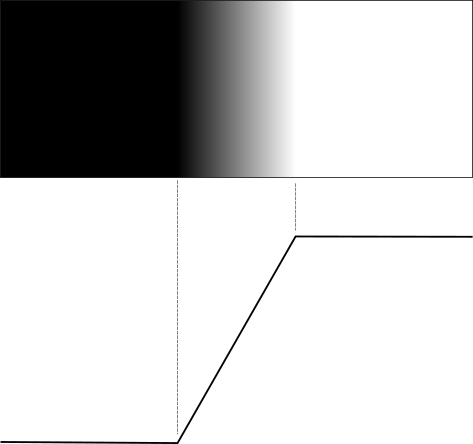
\includegraphics[width=6cm]{resources/inkscape/gradient.png}
    \end{center}
    \caption{Intensity of a signal with an edge.}
    \label{fig:edge_intensities}
\end{figure}

\subsection{Calculating gradient}

The first common way of working out where the edge is located is by looking at
the gradient of the image. The gradient of an image $\nabla f(x,y)$ is defined
as a vector \cite{gonzalez2002}:
$$\nabla f =
\begin{bmatrix}
    \dfrac{\partial f}{\partial x}\\[2ex]
    \dfrac{\partial f}{\partial y}
\end{bmatrix}$$
This vector represents the rate of change in the image intensities, and it points in
the direction of the maximum rate of change of intensity. Often just the bare
vector is not of interest; instead, the magnitude of the gradient, denoted as
$\nabla f$, is calculated too. Confusingly enough, sometimes this is also called
the gradient in the literature, but here I will differentiate it using the bold
text. Formally it is defined as:
$$|\nabla f| = \text{mag}(\nabla f) = \sqrt{(\frac{\partial f}{\partial x})^2 +
\frac{\partial f}{\partial y}^2}$$

Now the question is how to calculate the partial derivatives of some digital image.
It is impossible to calculate the partial derivatives using the standard
definition from mathematical analysis because digital images are discrete; thus,
we must use an approximation. To calculate the $\frac{\partial f}{\partial x}$
we can use the following approximation:
$$\frac{\partial f}{\partial x} \approx f(i+1,j)-f(i-1,j)$$
and similarly for the $\frac{\partial f}{\partial y}$ we can use:
$$\frac{\partial f}{\partial y} \approx f(i, j+1)-f(i,j-1)$$

This provides a reasonable approximation of the gradient. An example of the
magnitude of the gradient is visible in Figure \textbf{TODO}.

\begin{itemize}
    \item Images
    \item Approx. formular for the mahnitude of the gradient
\end{itemize}

\subsection{Laplacian operator}

The second common way of finding edges is using the second derivative, or more
precisely using the Laplacian. For a 2D function $f(x, y)$ the Laplacian is
defines as \cite{gonzalez2002}:

$$\nabla^2 f = \frac{\partial^2 f}{\partial x^2} + \frac{\partial^2 f}{\partial y^2}$$

However, in the context of digital image processing our signal is discrete;
therefore, a discrete approximation is needed. A fairly standard way is to use
the following approach to calculate the partial second derivative in the $x$
axis:
$$\frac{\partial^2 f}{\partial x^2} = f(i + 1, j) + f(i - 1, j) - 2f(i, j)$$
and similar in the y axis:
$$\frac{\partial^2 f}{\partial y^2} = f(i, j + 1) + f(i, j - 1) - 2f(i, j)$$
Substituting into the prior definition we get the following approximation:
$$\nabla^2 f = f(i+1, j) + f(i-1, j) + f(i, j+1) + f(i, j-1) - 4f(i,j)$$
To calculate the Laplacian of an image, this formula is applied to every pixel.

% todo insert an image and description
% todo insert and examplorary image

\begin{figure}
    \begin{center}
        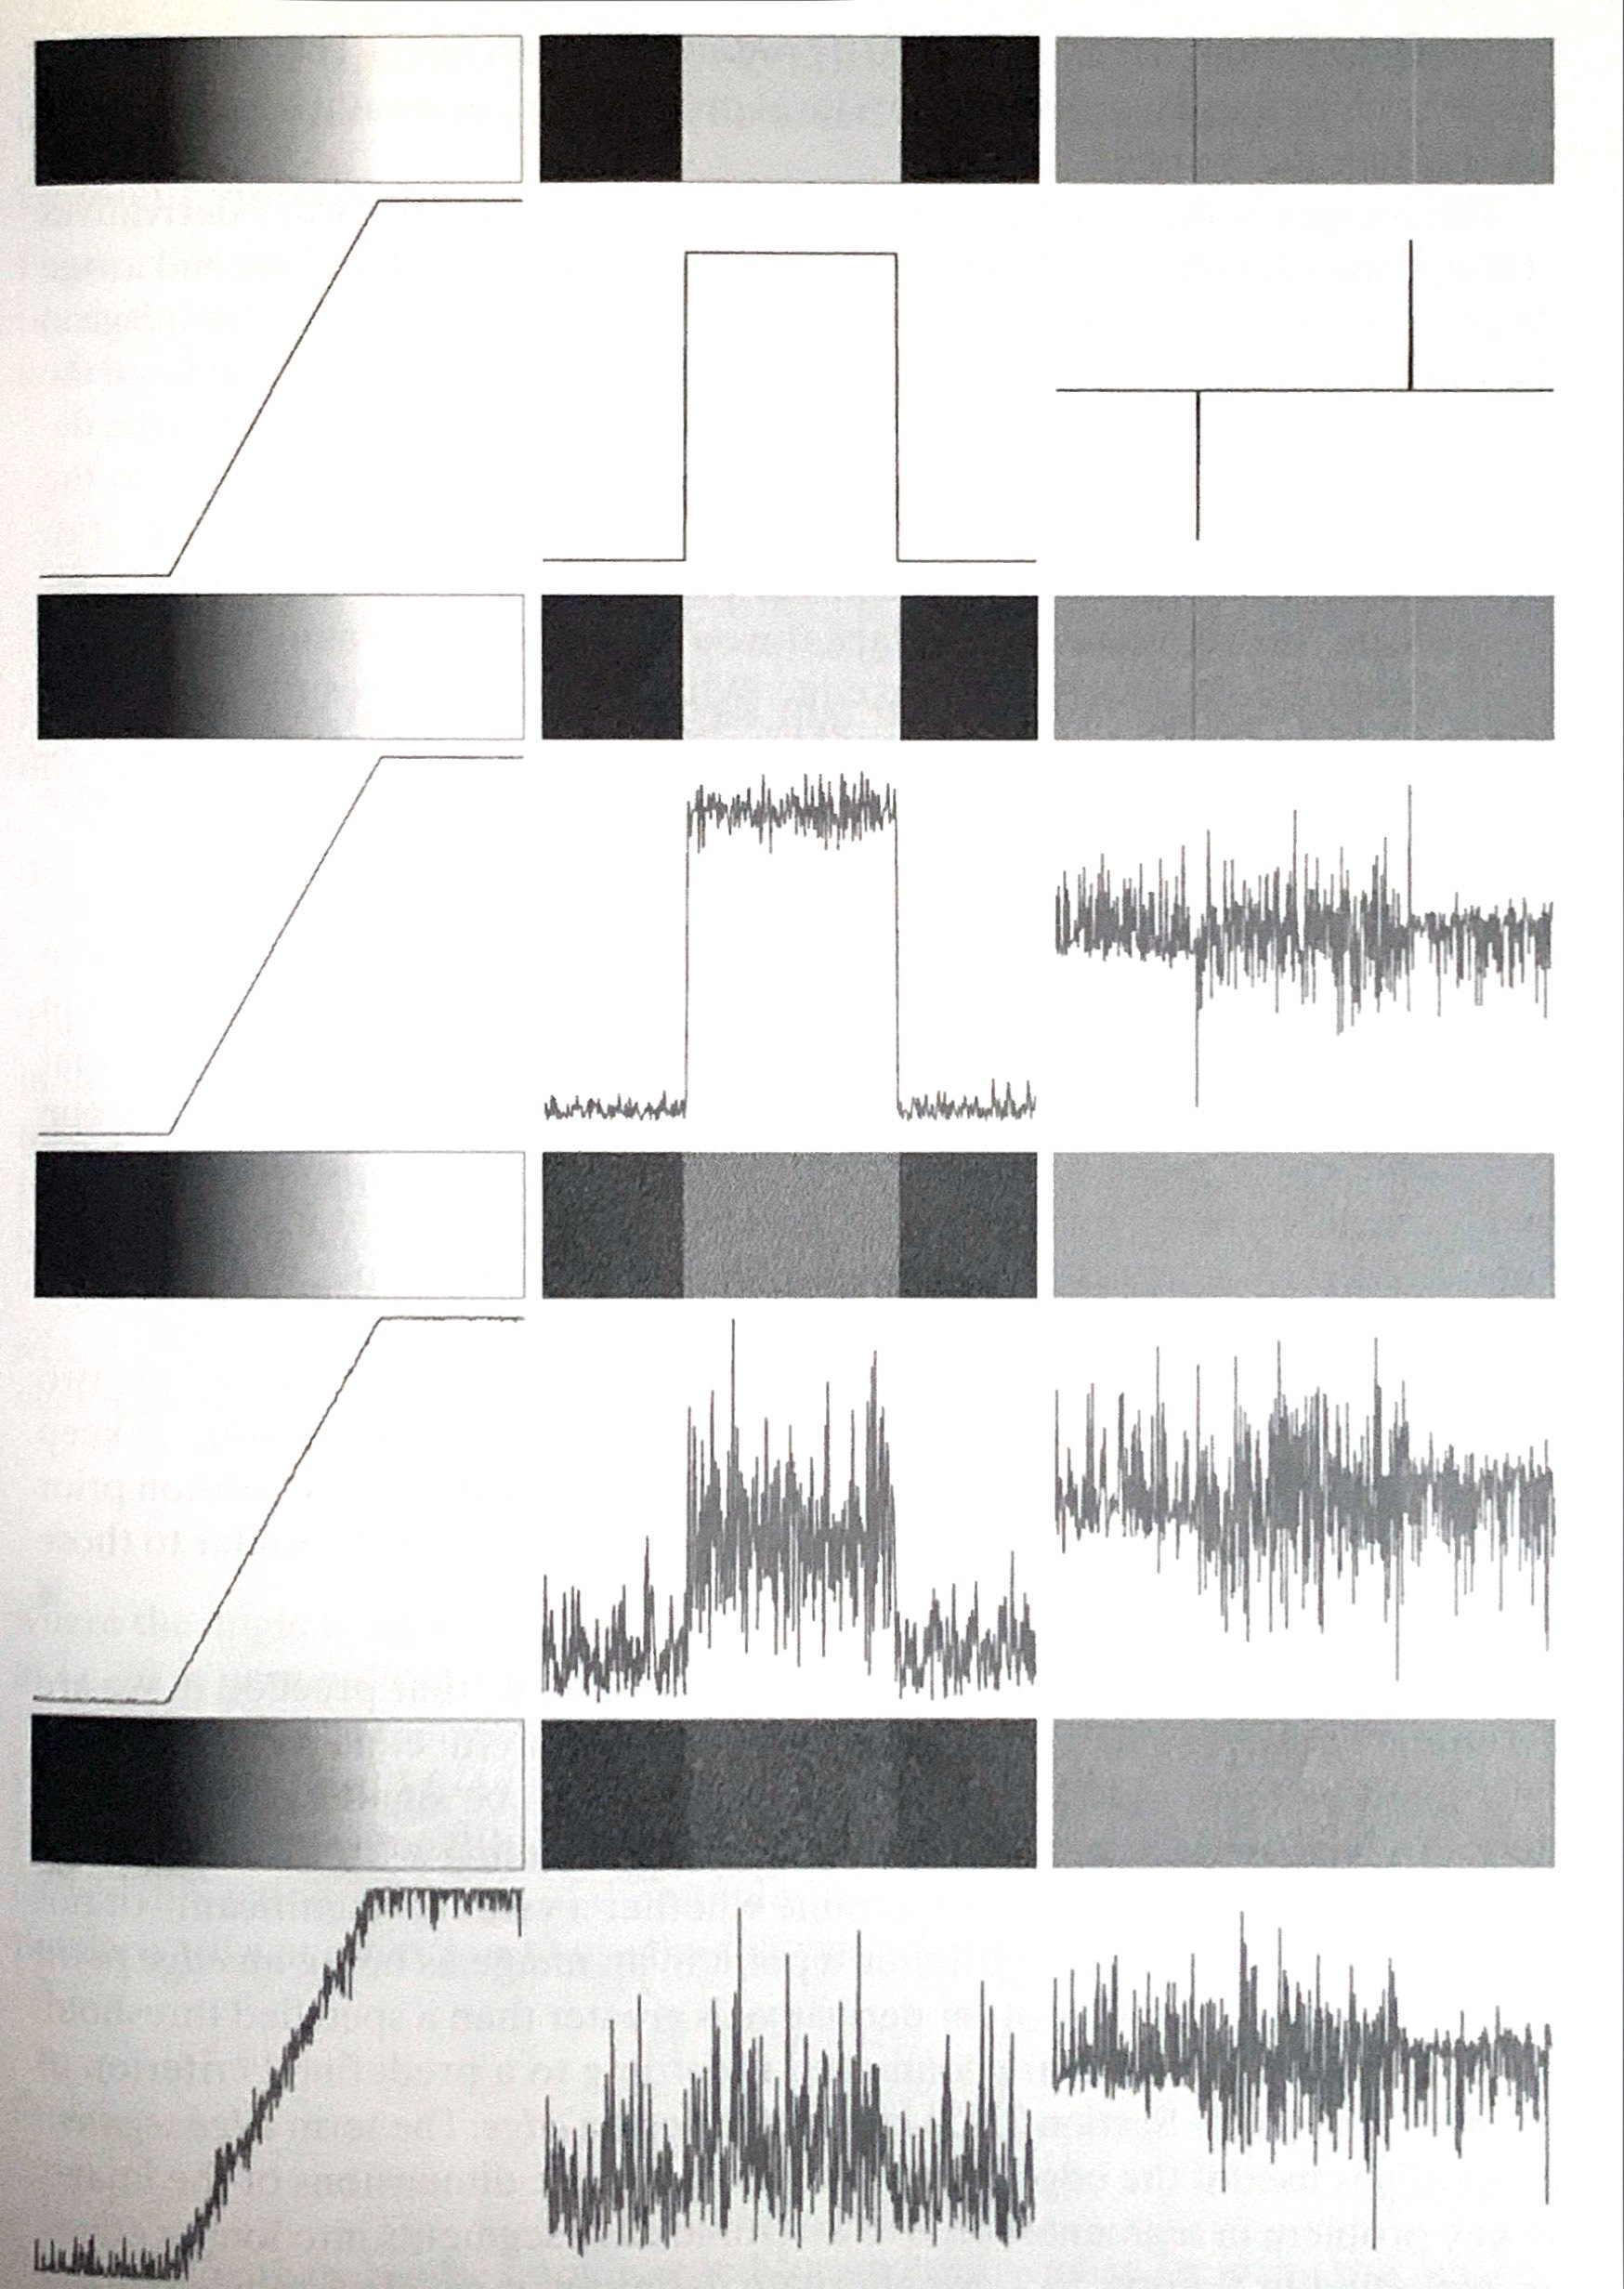
\includegraphics[width=6cm]{"resources/gonzalez_edges_and_noise.jpg"}
    \end{center}
    \caption{Effect of noise on signal \cite{gonzalez2002}}
    \label{fig:edges_noise}
\end{figure}

One of the disadvantages of this approach is the sensitivity to noise. For
demonstration purposes, the effects are shown in 1D in Figure
\ref{fig:edges_noise}. While the original
signal does not look too degraded, it is impossible to find the correct
zero-crossings. Therefore we have to help the operator by first smoothing the
image. A common approach is to first use Gaussian smoothing; this is sometimes
called a Laplacian of Gaussian operator or a Mexican hat filer. The idea is that
by averaging, we reduce some of the effects of the noise
\cite{hipr-mexican-hat}. The Figure \textbf{TODO} demonstrates this effect.

Since the Laplacian is based on second derivatives, it has the property that
each edge produces a zero crossing. This can be readily utilised to find edges
inside an image. A simple algorithm is to go through the whole image and check
if a particular pixel at a given position is positive while its neighbours are
negative. If this condition is true, we set this position to white in the
resulting image and black otherwise. This creates an TODO. Here another valuable
property of the zero-crossing algorithm can be seen. The produced edges are
thin, and form closed contours.

\section{Thresholding}

\subsection{Otsu method}

The Otsu thresholding method is a popular technique to determine a threshold
value between two classes (usually the foreground and the background). As such,
it works well if the image's histogram has a clear bimodal distribution. The
main idea of this approach is to see the problem of finding the threshold as an
optimization problem, where the inter-class variance of the two classes is to be
minimized. More information is available in the paper \cite{otsu1979}.

\begin{figure}
    \begin{subfigure}[t]{0.45\textwidth}
        \centering
        \frame{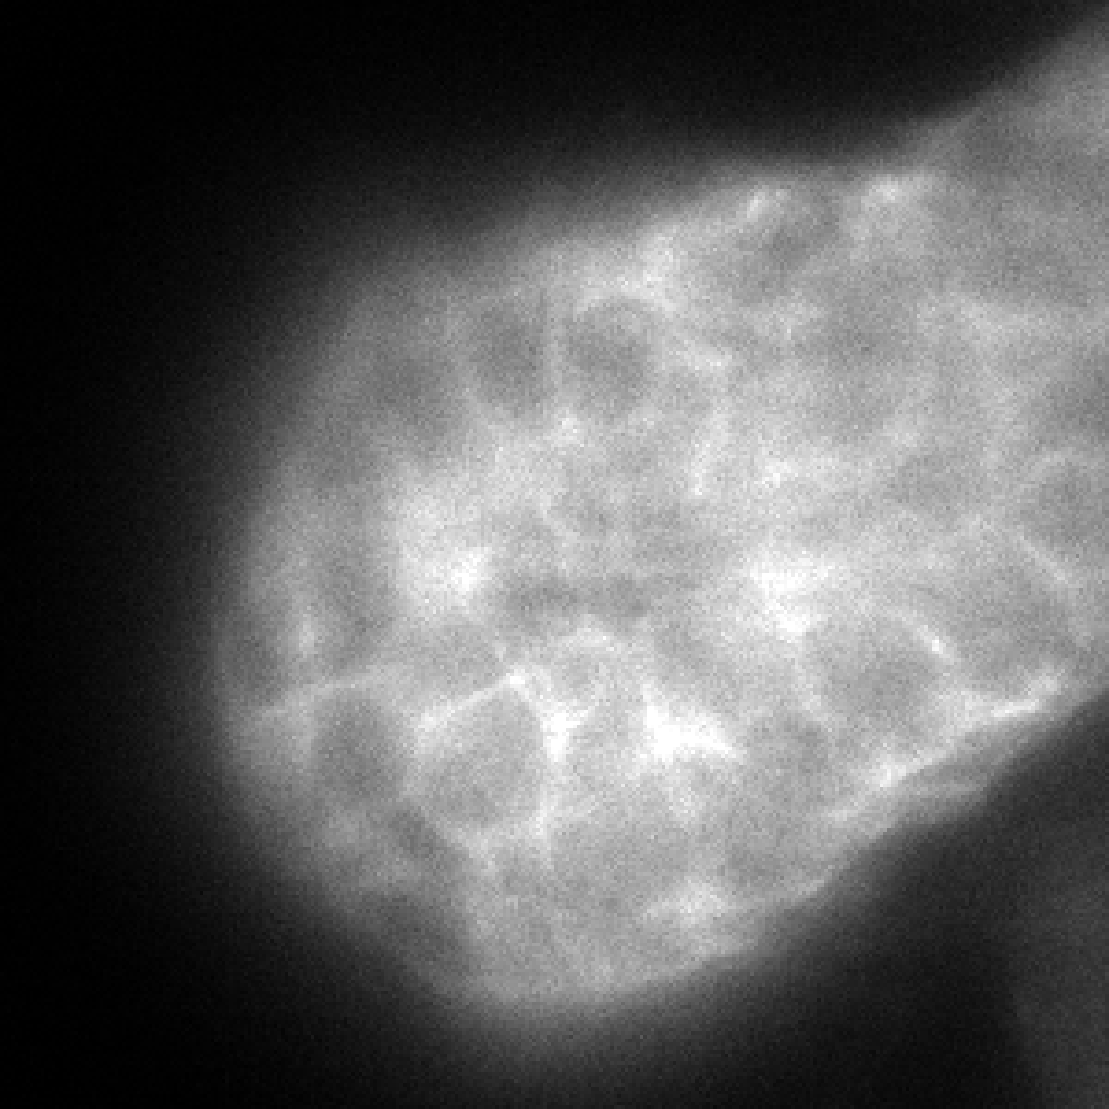
\includegraphics[width=\textwidth]{resources/otsu-orig.png}}
        \caption{Image from membrane-stained channel.}
        \label{fig:otsu-orig}
    \end{subfigure}
    \begin{subfigure}[t]{0.45\textwidth}
        \centering
        \frame{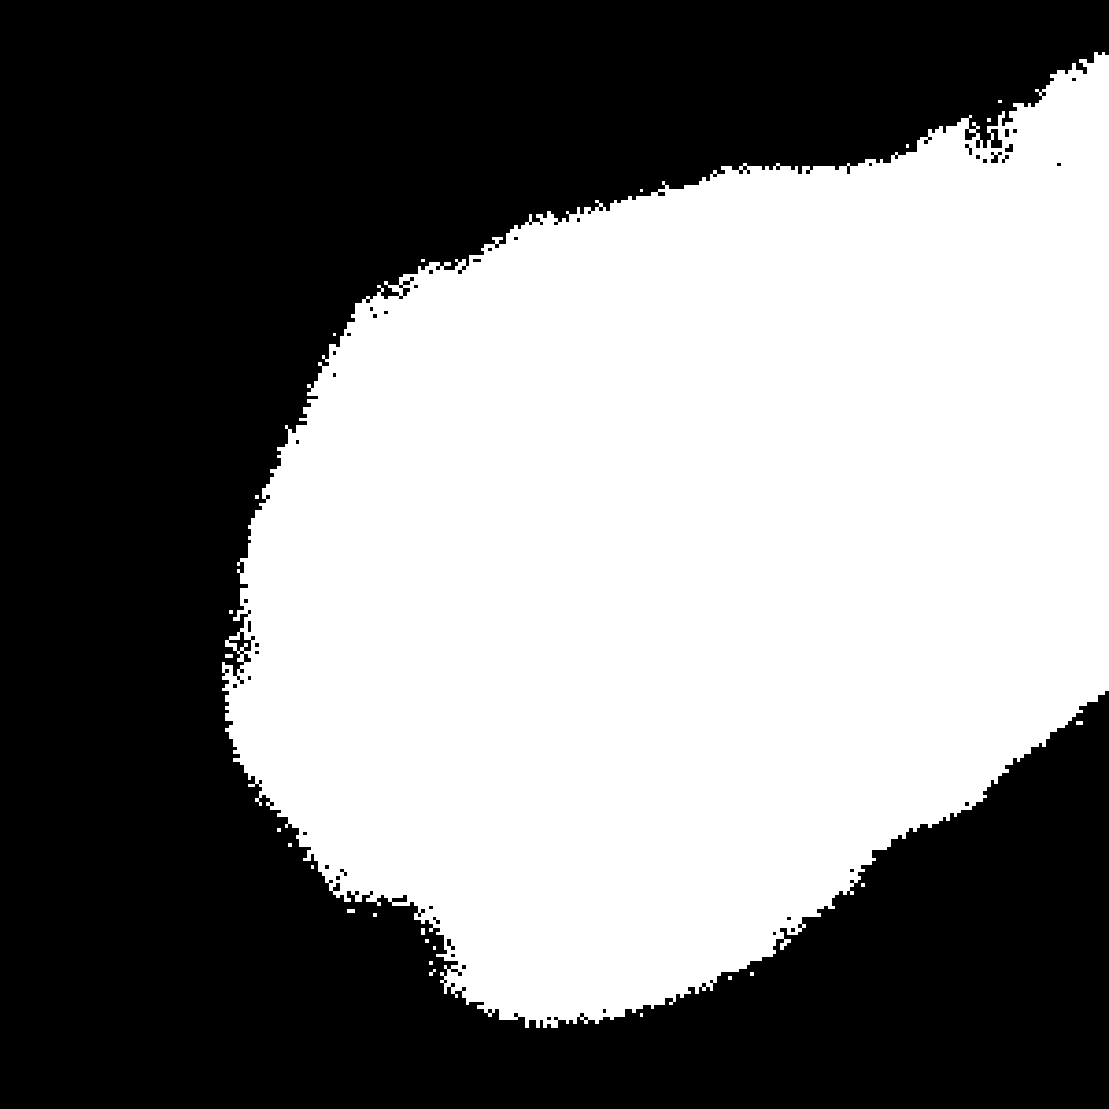
\includegraphics[width=\textwidth]{resources/otsu-thresholded.png}}
        \caption{Thresholded image.}
        \label{fig:otsu-thresholded}
    \end{subfigure}
    \begin{subfigure}[t]{0.6\textwidth}
        \centering
        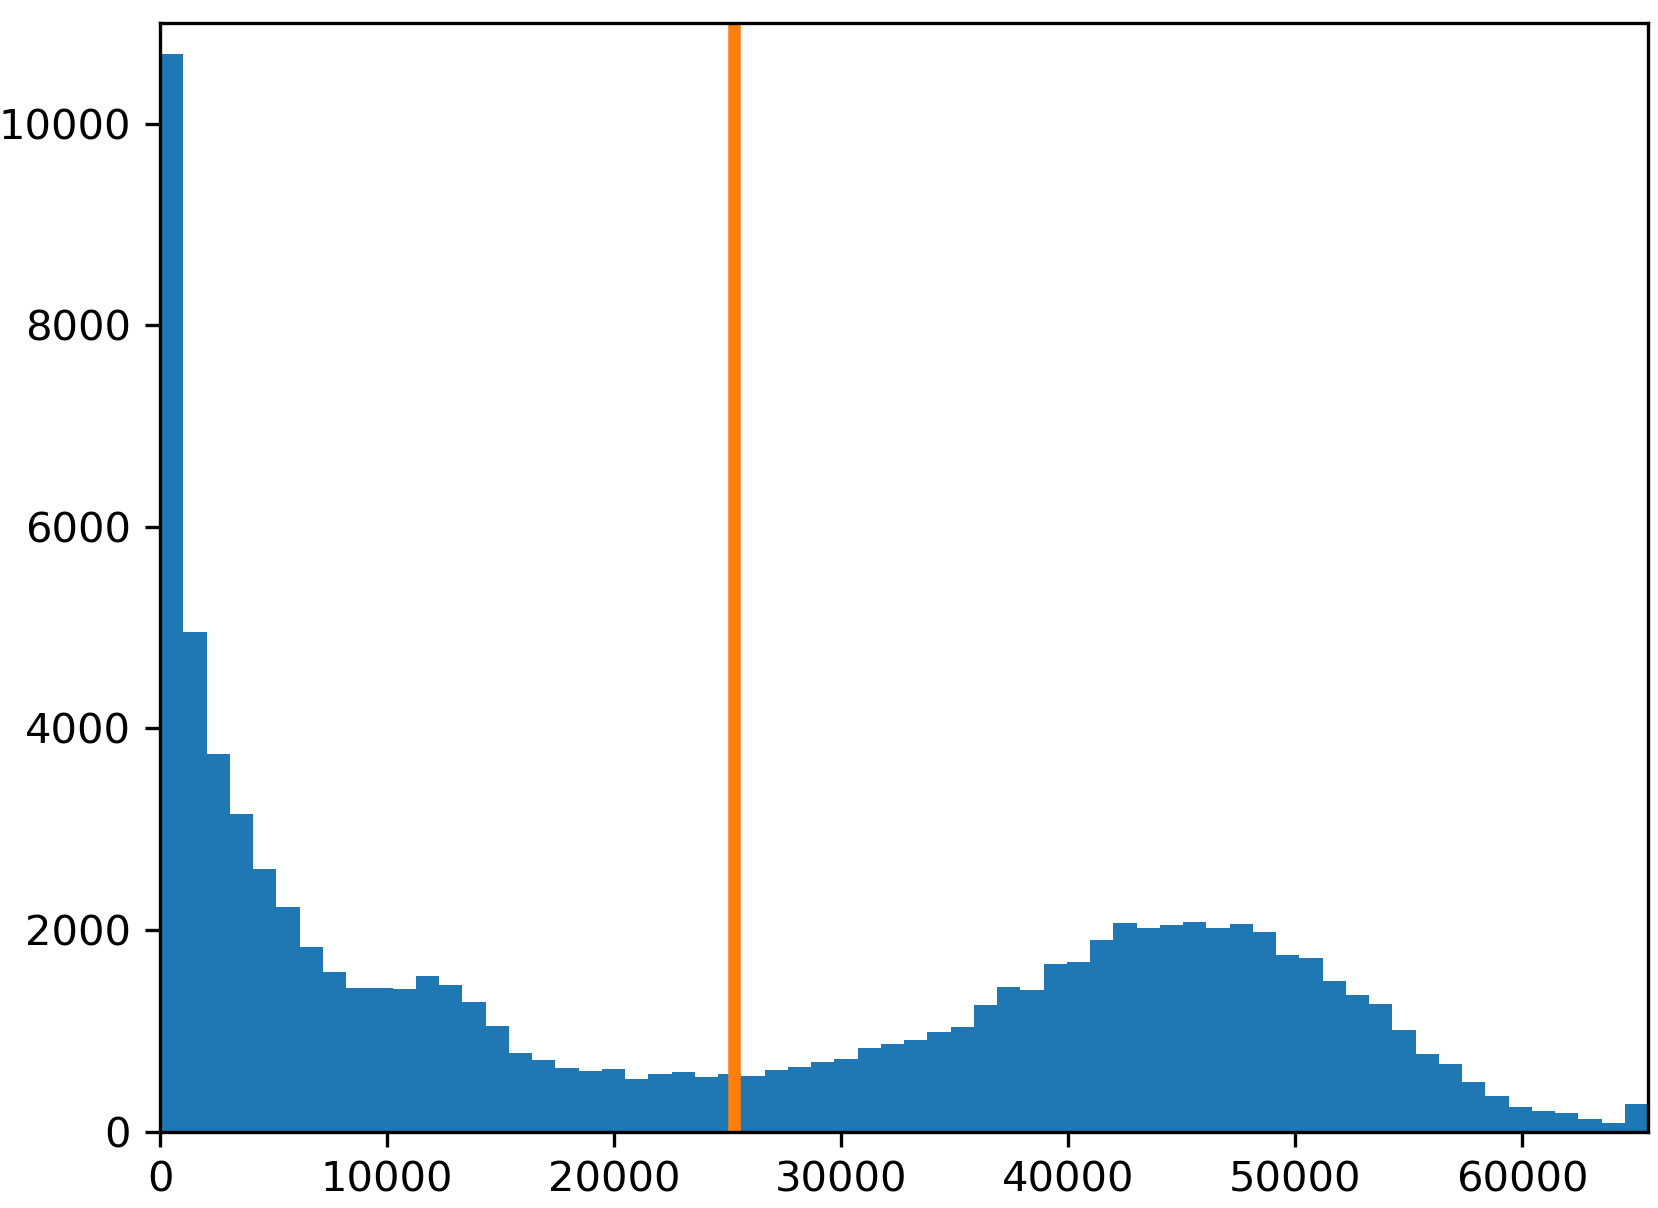
\includegraphics[width=\textwidth]{resources/otsu-histogram.png}
        \caption{Histogram of the image, with a line indicating the threshold.}
        \label{fig:otsu-histogram}
    \end{subfigure}
    \caption{Demonstration of the otsu thresholding method.}
    \label{fig:opening}
\end{figure}

\subsection{Gradient threshold}

Another useful thresholding method is the gradient threshold algorithm. Unlike
many other thresholding algorithms, it does not purely rely on the analysis of
the image's histogram; instead, the threshold is calculated as a weighted sum of
the image's intensities, where the weights are dictated by the magnitude of the
gradient \cite{pb130}.

The idea is that the background tends to be rather uniform compared to the
object in the foreground; hence, the magnitude of the gradient is the greatest
in the foreground, and the edge separating it from the background. That can be
utilized by using the magnitude as the weight in the summing of intensities.
This way the background's intensities play lesser role.

Formally the threshold $a$ is defined as:
$$a = \sum_{u, v} I(u, v) \frac{|\nabla I(u, v)|}{\sum_{i, j} |\nabla(i,j)|}$$
where $I(i, j)$ stands for the image intensity at the $(i, j)$ position.

\begin{figure}
    \begin{center}
        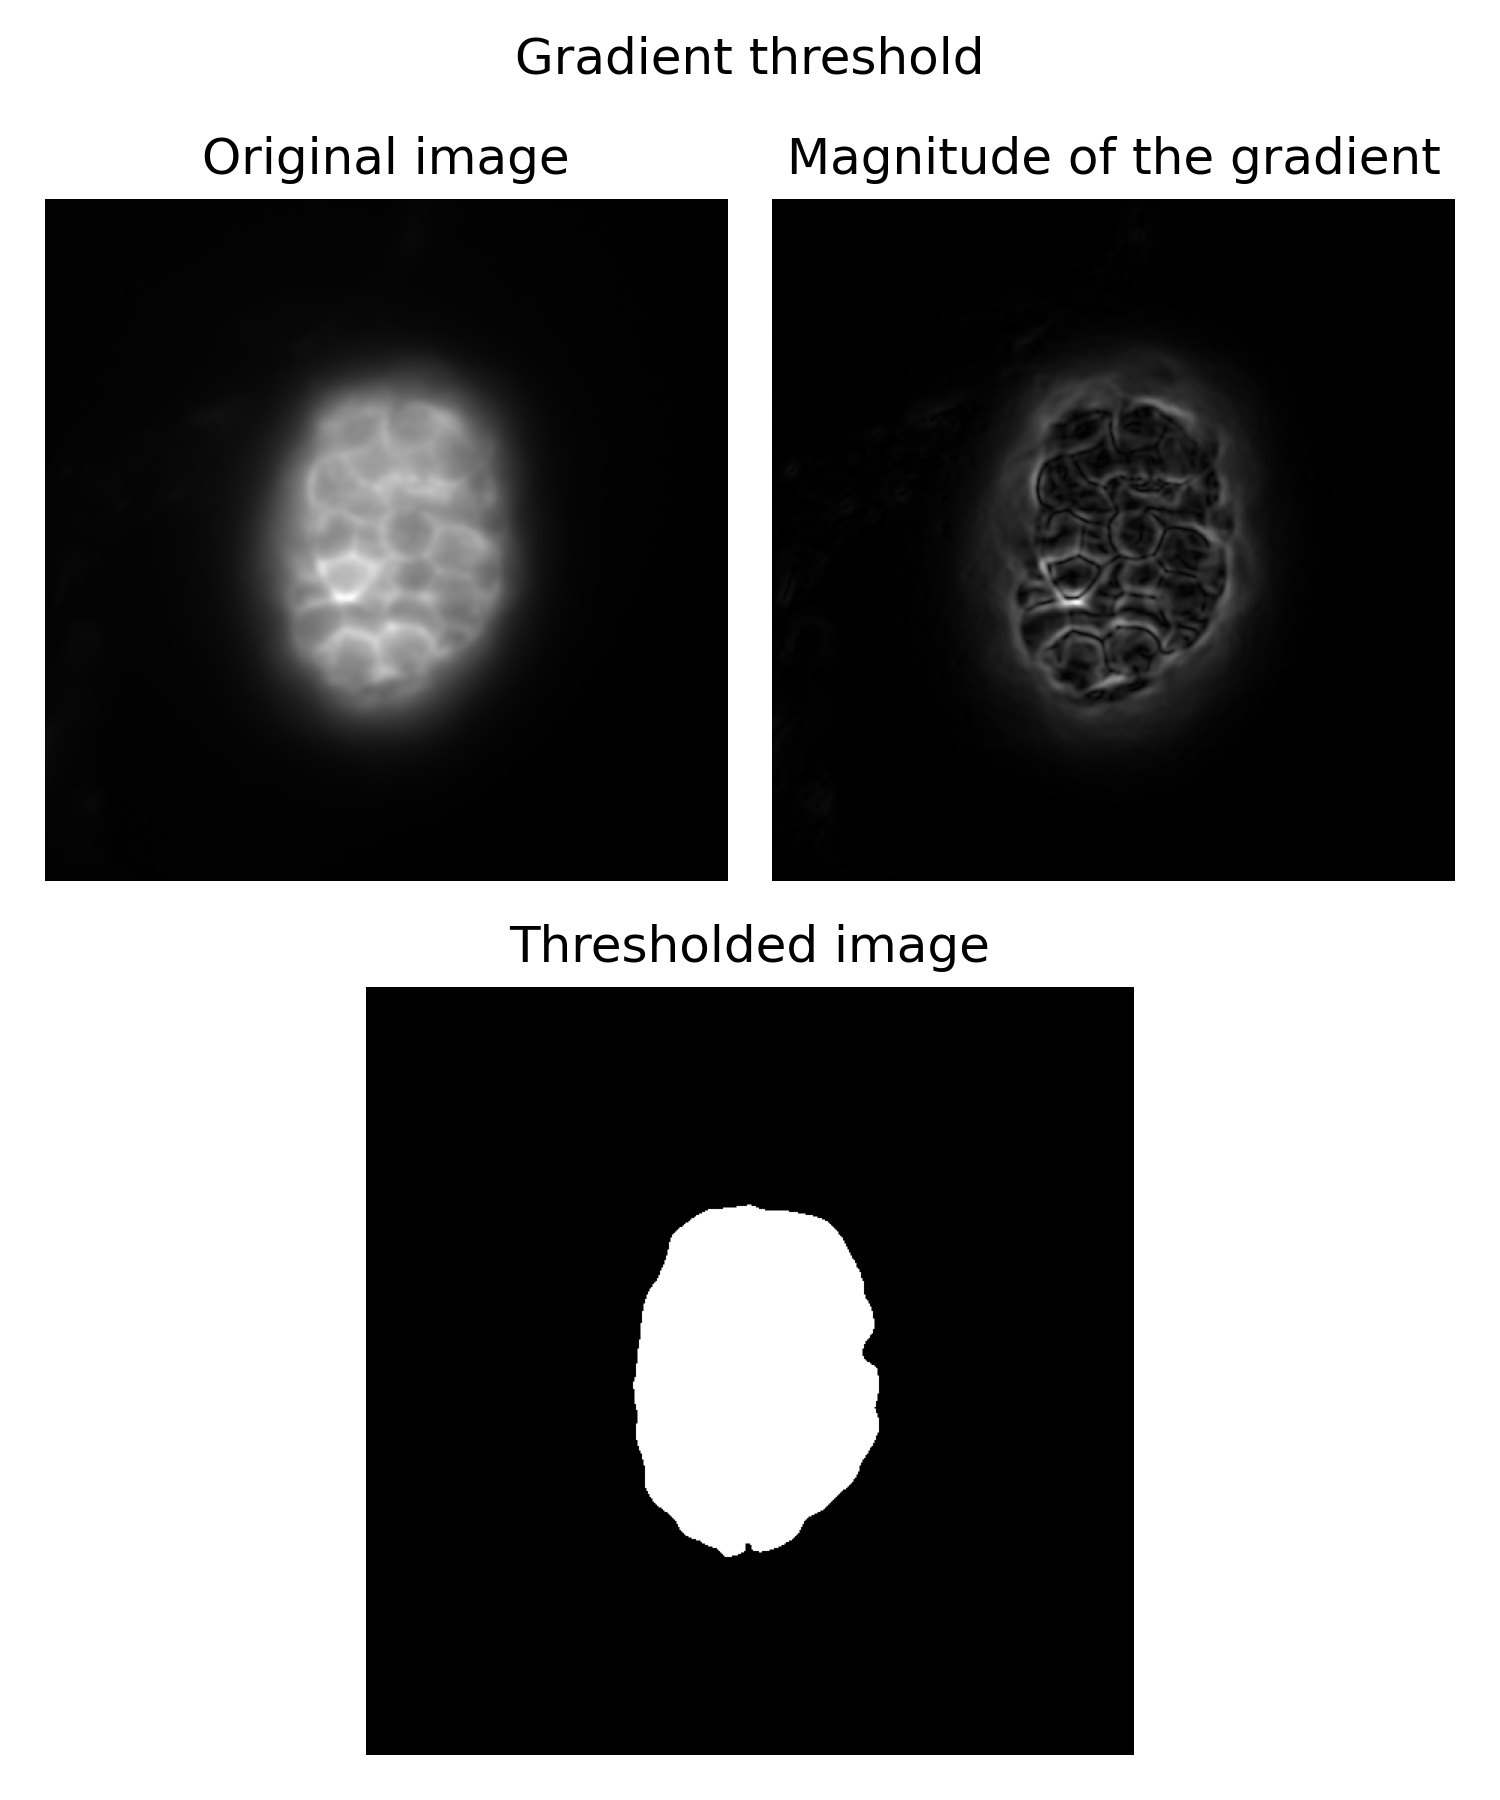
\includegraphics[width=8cm]{"resources/demo-gradient-threshold.png"}
    \end{center}
    \caption{Demo of gradient threshold.}
    \label{fig:demo_grad_thresh}
\end{figure}

In Figure \ref{fig:demo_grad_thresh} an example image is shown. There, the
gradient thresholding algorithm was used to segment the cell from the
background. As can be seen, the magnitude of the gradient is biggest in the
cell; hence, it contributes more to the value of the threshold.

\textbf{TODO: Why this threshold method is useful}

\section{Mathematical morphology}

Mathematical morphology is an area of research studying how to extract valuable
information and how to filter images. Few examples of what mathematical
morphology study are edge-detecting algorithms, finding convex hulls, and image
filtering. In the simplest terms, mathematical morphology looks at images as
sets of numbers and modifies them using structural elements. Those can take many
forms, but their shape varies based on the task we are trying to achieve. The
main use of mathematical morphology in this thesis is to pre- and post-process
image data generated by other image processing methods. First, some basic
operations on binary images are described. Note that this area is vast and still
being actively researched, and I will cover only parts which are helpful later
in my prototype.

In this branch of image processing, we look at the images through set theory
instead of looking at images as discrete-valued functions. In this context, an
image is a subset of 2-D integer space $\Z^2$, which can easily be generalized
to more dimensions. Each element of this subset $(x, y)$ represents a present
pixel at those coordinates in the image. In other words, if we look at an image
as an array of rectangular shape, then each foreground pixel's coordinates will
be included in the set representation.

\subsection{Preliminary}
Before we look at the two main operations --- erosion and dilation --- we have to
define two not-so-common operations on sets which are heavily used in
mathematical morphology.

During the following sections, we need to be able to talk about how to create a
reflection of the image around its origin, as shown in Figure
\ref{fig:morp_refl}. Reflection  of a set $B$ is formally defined as \cite{gonzalez2002}:
$$\hat{B} = \{w | w=-b \text{ , for } b \in B\}$$
\begin{figure}
    \begin{center}
        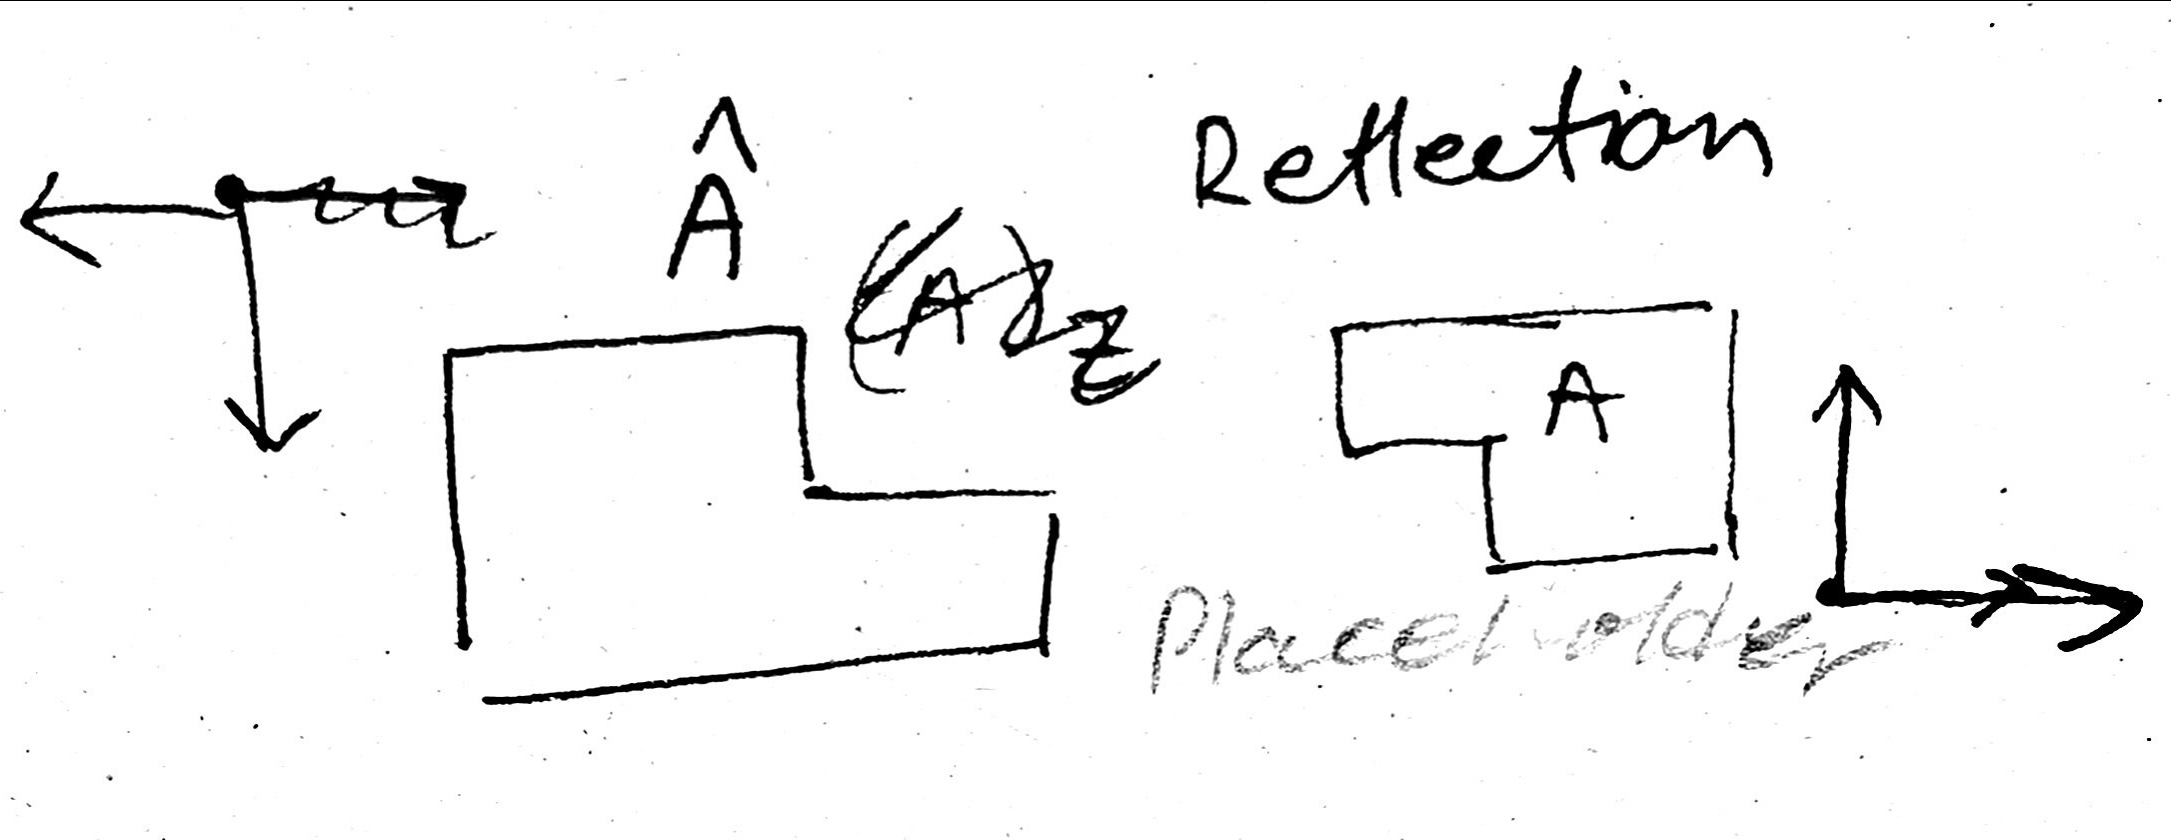
\includegraphics[width=6.3cm]{resources/morph_reflection.jpg}
    \end{center}
    \caption{Morphological reflection} % todo: replace
    \label{fig:morp_refl}
\end{figure}

While manipulating images we commonly have to move parts of the image around.
In principle, a similar operation, called translation, is defined on sets. The
formal definition of moving a set $A$ by some translation vector $z$ is
\cite{gonzalez2002}:
$$(A)_z = \{c | c = a + z\text{ , for } a \in A\}$$
The operation is illustrated in Figure \ref{fig:morph_translation} where the set
$A$ is moved downwards by a vector $z$.
\begin{figure}
    \begin{center}
        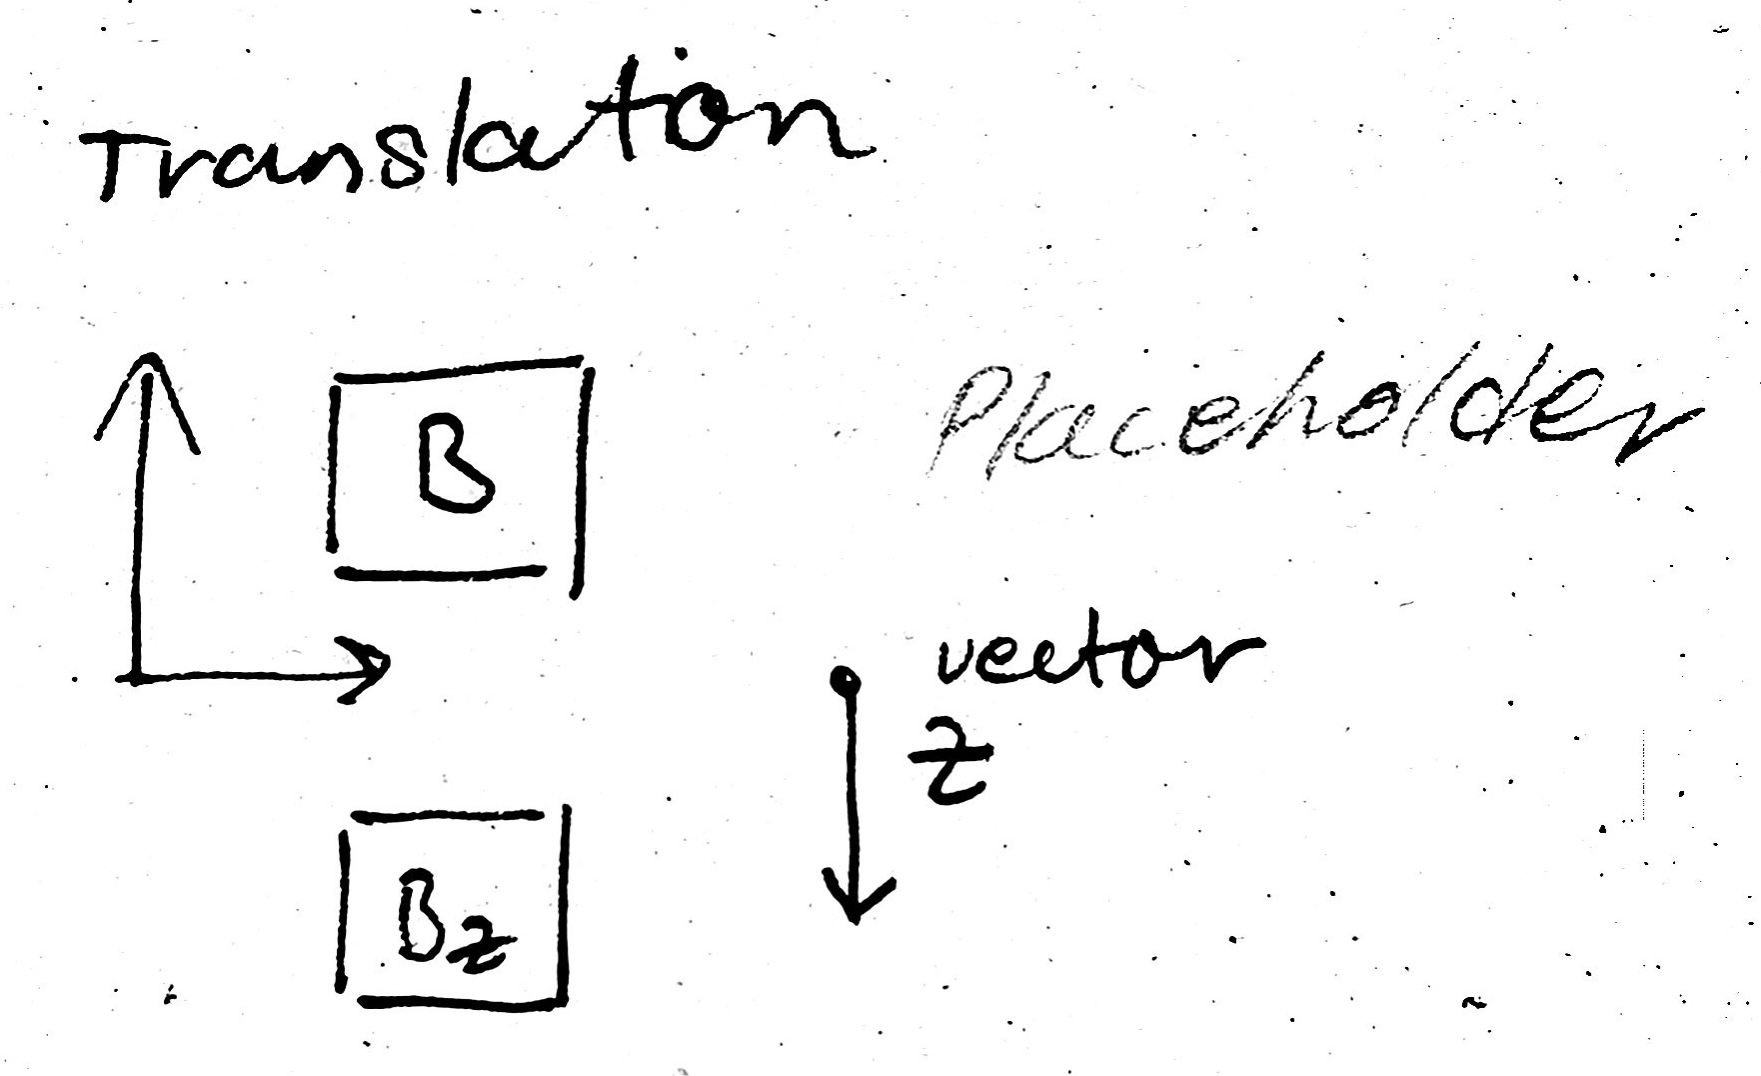
\includegraphics[width=6.3cm]{resources/morph_translation.jpg}
    \end{center}
    \caption{Morphological translation} % todo: Replace
    \label{fig:morph_translation}
\end{figure}

\subsection{Dilation and Erosion}
Now it is possible to properly define two fundamental operations in the field of
mathematical morphology, upon which many other operations are built. Both of
these operations include a structural element. A structural element is again a
set, but it can be used to describe how far and in which way a particular
operation will influence the result.


\subsubsection{Dilation}
Intuitively we can think about the dilation operator as a way to dilate spots
inside an image into a bigger space. Formally it is defined as
\cite{gonzalez2002}
$$A \oplus B = \{z | (\hat{B}_z) \cap A \neq \emptyset\}$$
where $A$ and $B$ are both sets in $\Z^2$.

An example of dilation can be seen in Figure \ref{fig:morph_dilation}. In the
first row, we have a square image with a side length of $d$ and a structuring
element whose side length is a fourth of the original. If we apply the dilation
operation on these two images, we get the one on the right. You can imagine
taking the smaller square and gliding it over the bigger one. If there is an
overlap, we can add the centre of the structural element to the result.

Closer to the mathematical definition, all possible translations are applied to
the structural element and if there is an overlap, we add the centre of the
structural element to the resulting set.

For example, this operation can be used to join disconnected segments in an
image by choosing a large enough structural element. Its size will depend on the
particular example and does not necessarily have to be of regular size.

\begin{figure}
    \begin{center}
        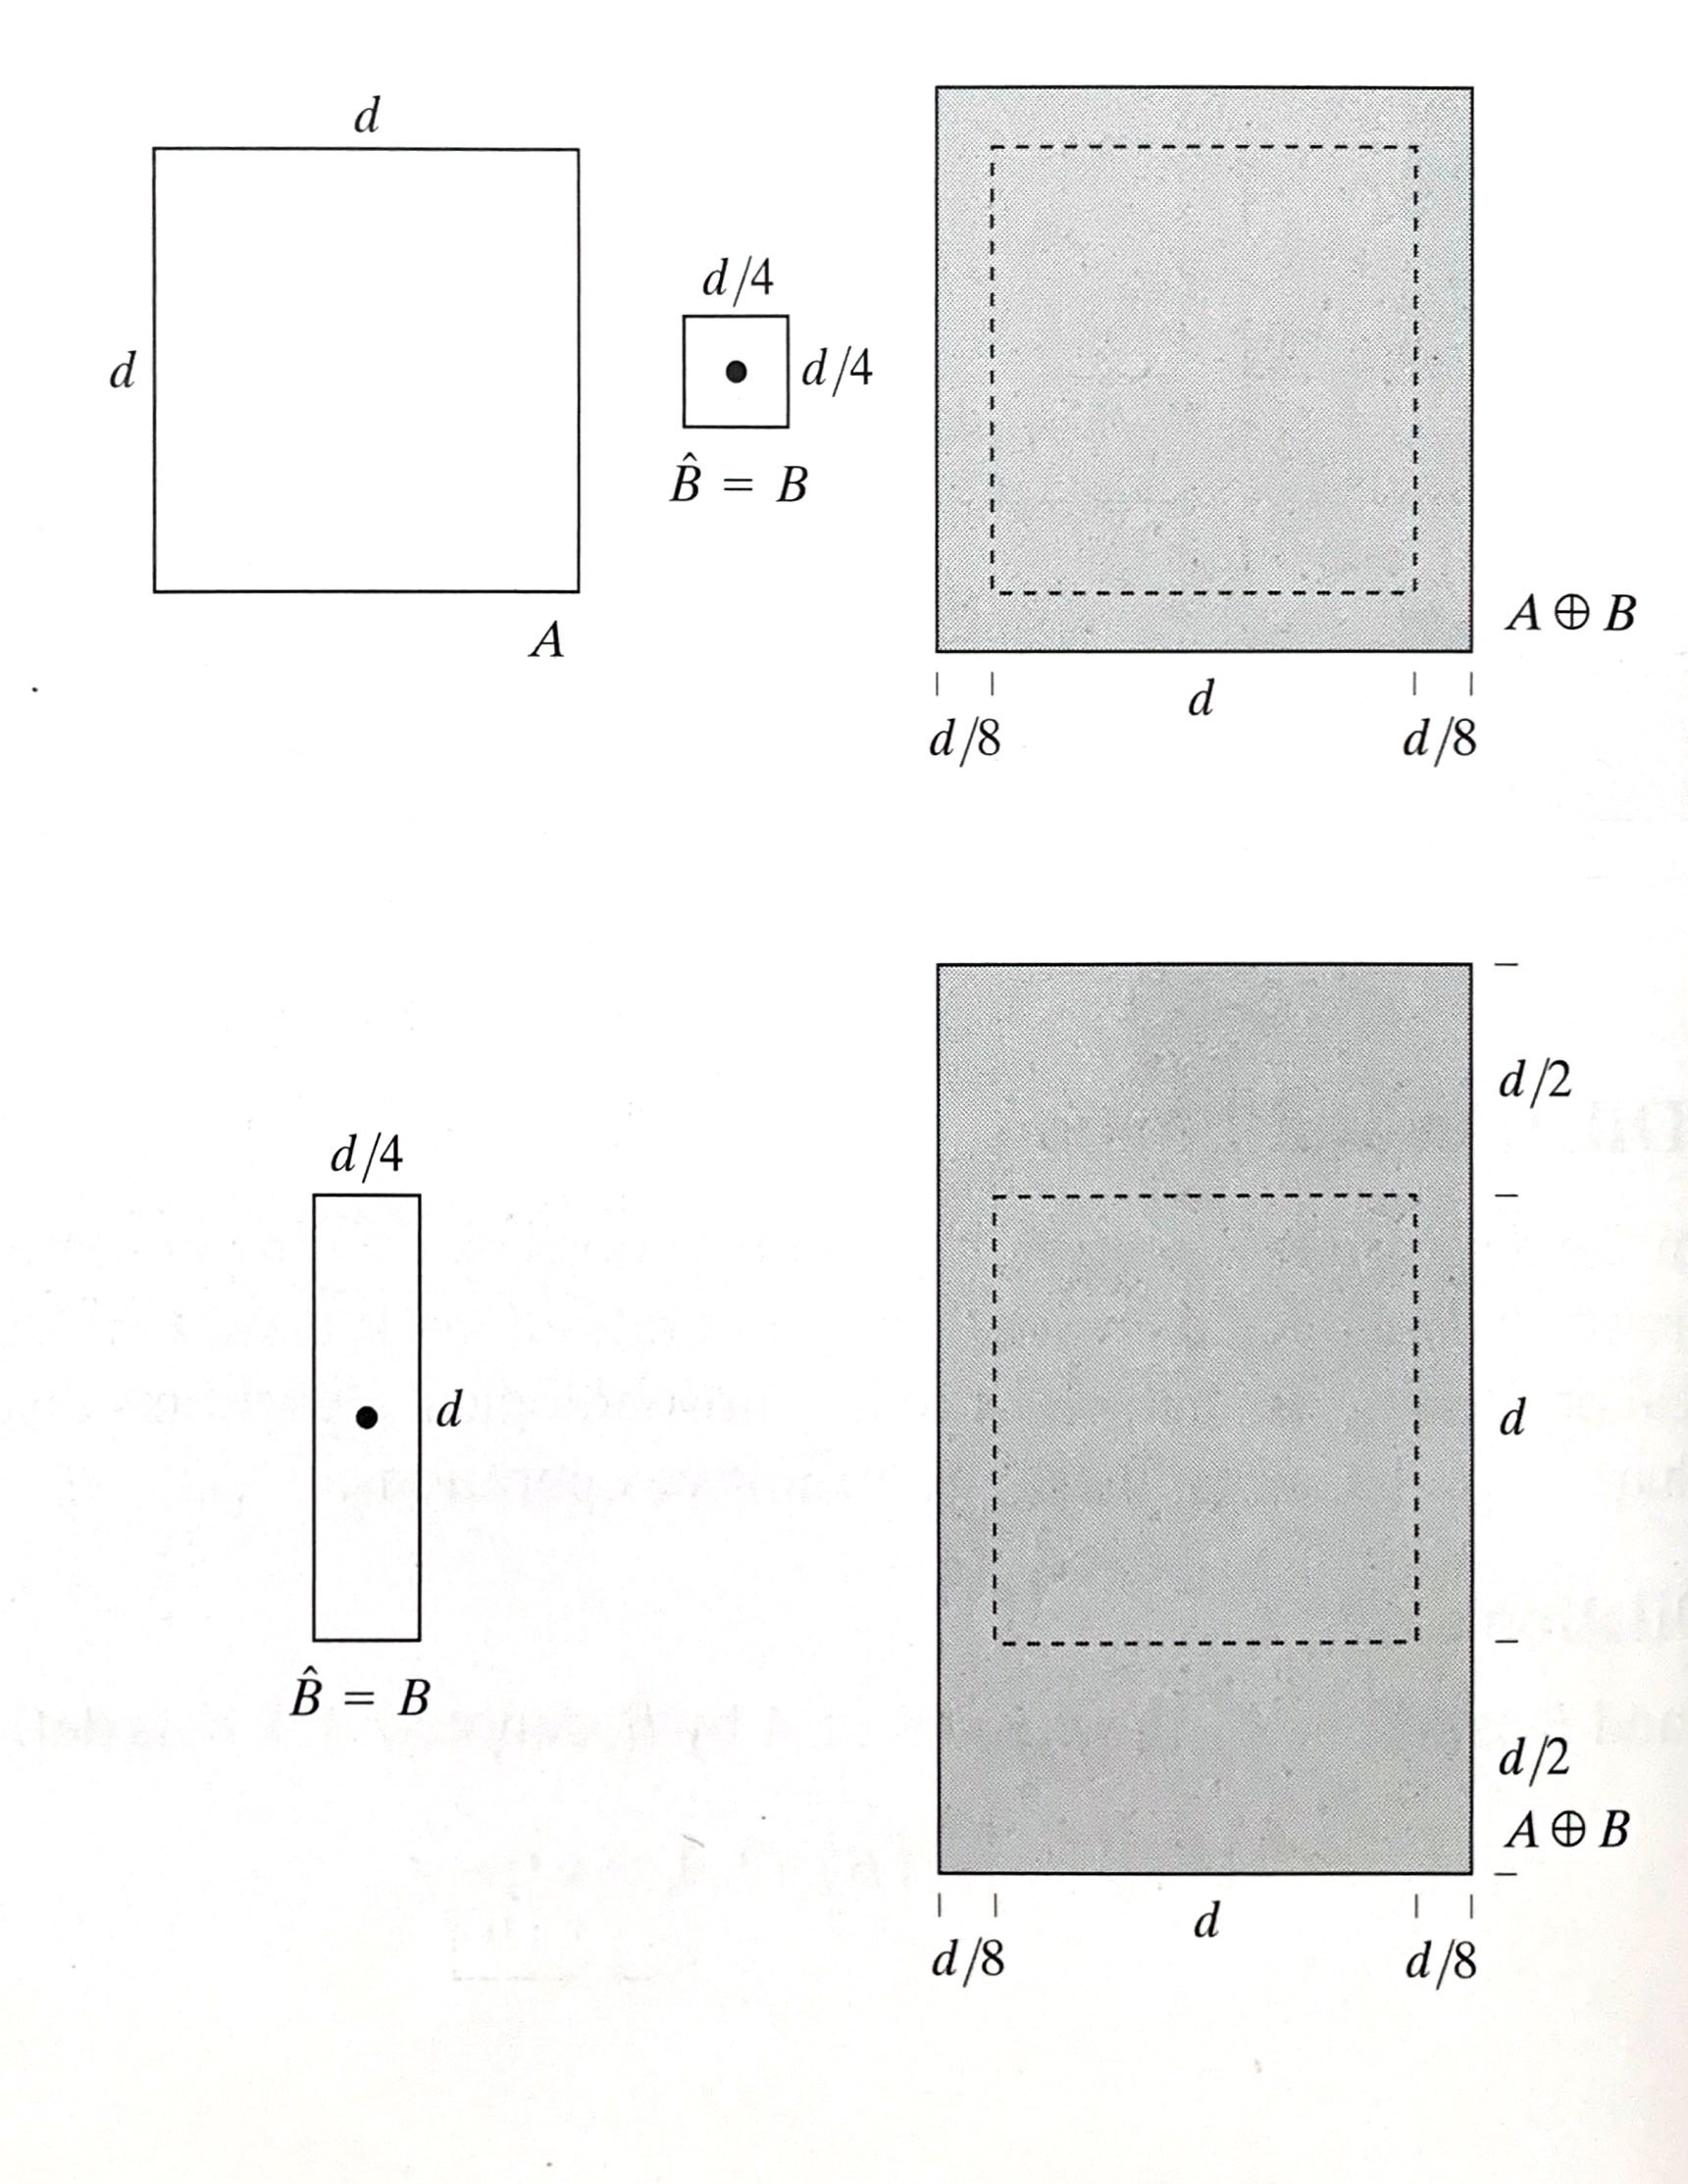
\includegraphics[width=6.3cm]{resources/morph_dilation.jpg}i
    \end{center}
    \caption{Morphological dilation (Gonzalez 2002)} % todo: Replace
    \label{fig:morph_dilation}
\end{figure}

\subsubsection{Erosion}

The next essential operation is erosion. As the name suggests, we use it to
erode parts of the image which we consider unnecessary. An erosion $A \ominus B$
of two sets $A$ and $B$, both being part of $\Z^2$ space, is defined as
\cite{gonzalez2002}: $$A \ominus B = \{z | (B)_z \subseteq A\}$$

Again $A$ can be thought of as an image while $B$ can be looked at as a
structural element. In contrast to the dilation operation, we are now looking if
the whole structural element fits inside $A$ as can be seen in Figure
\ref{fig:morph_erosion}. There a smaller structural element is used to cut away
parts of the bigger square.

As opposed to the dilation, we can use erosion to divide lightly connected
segments, and to suppress noise and other unwanted disturbances in an image.

\begin{figure}
    \begin{center}
        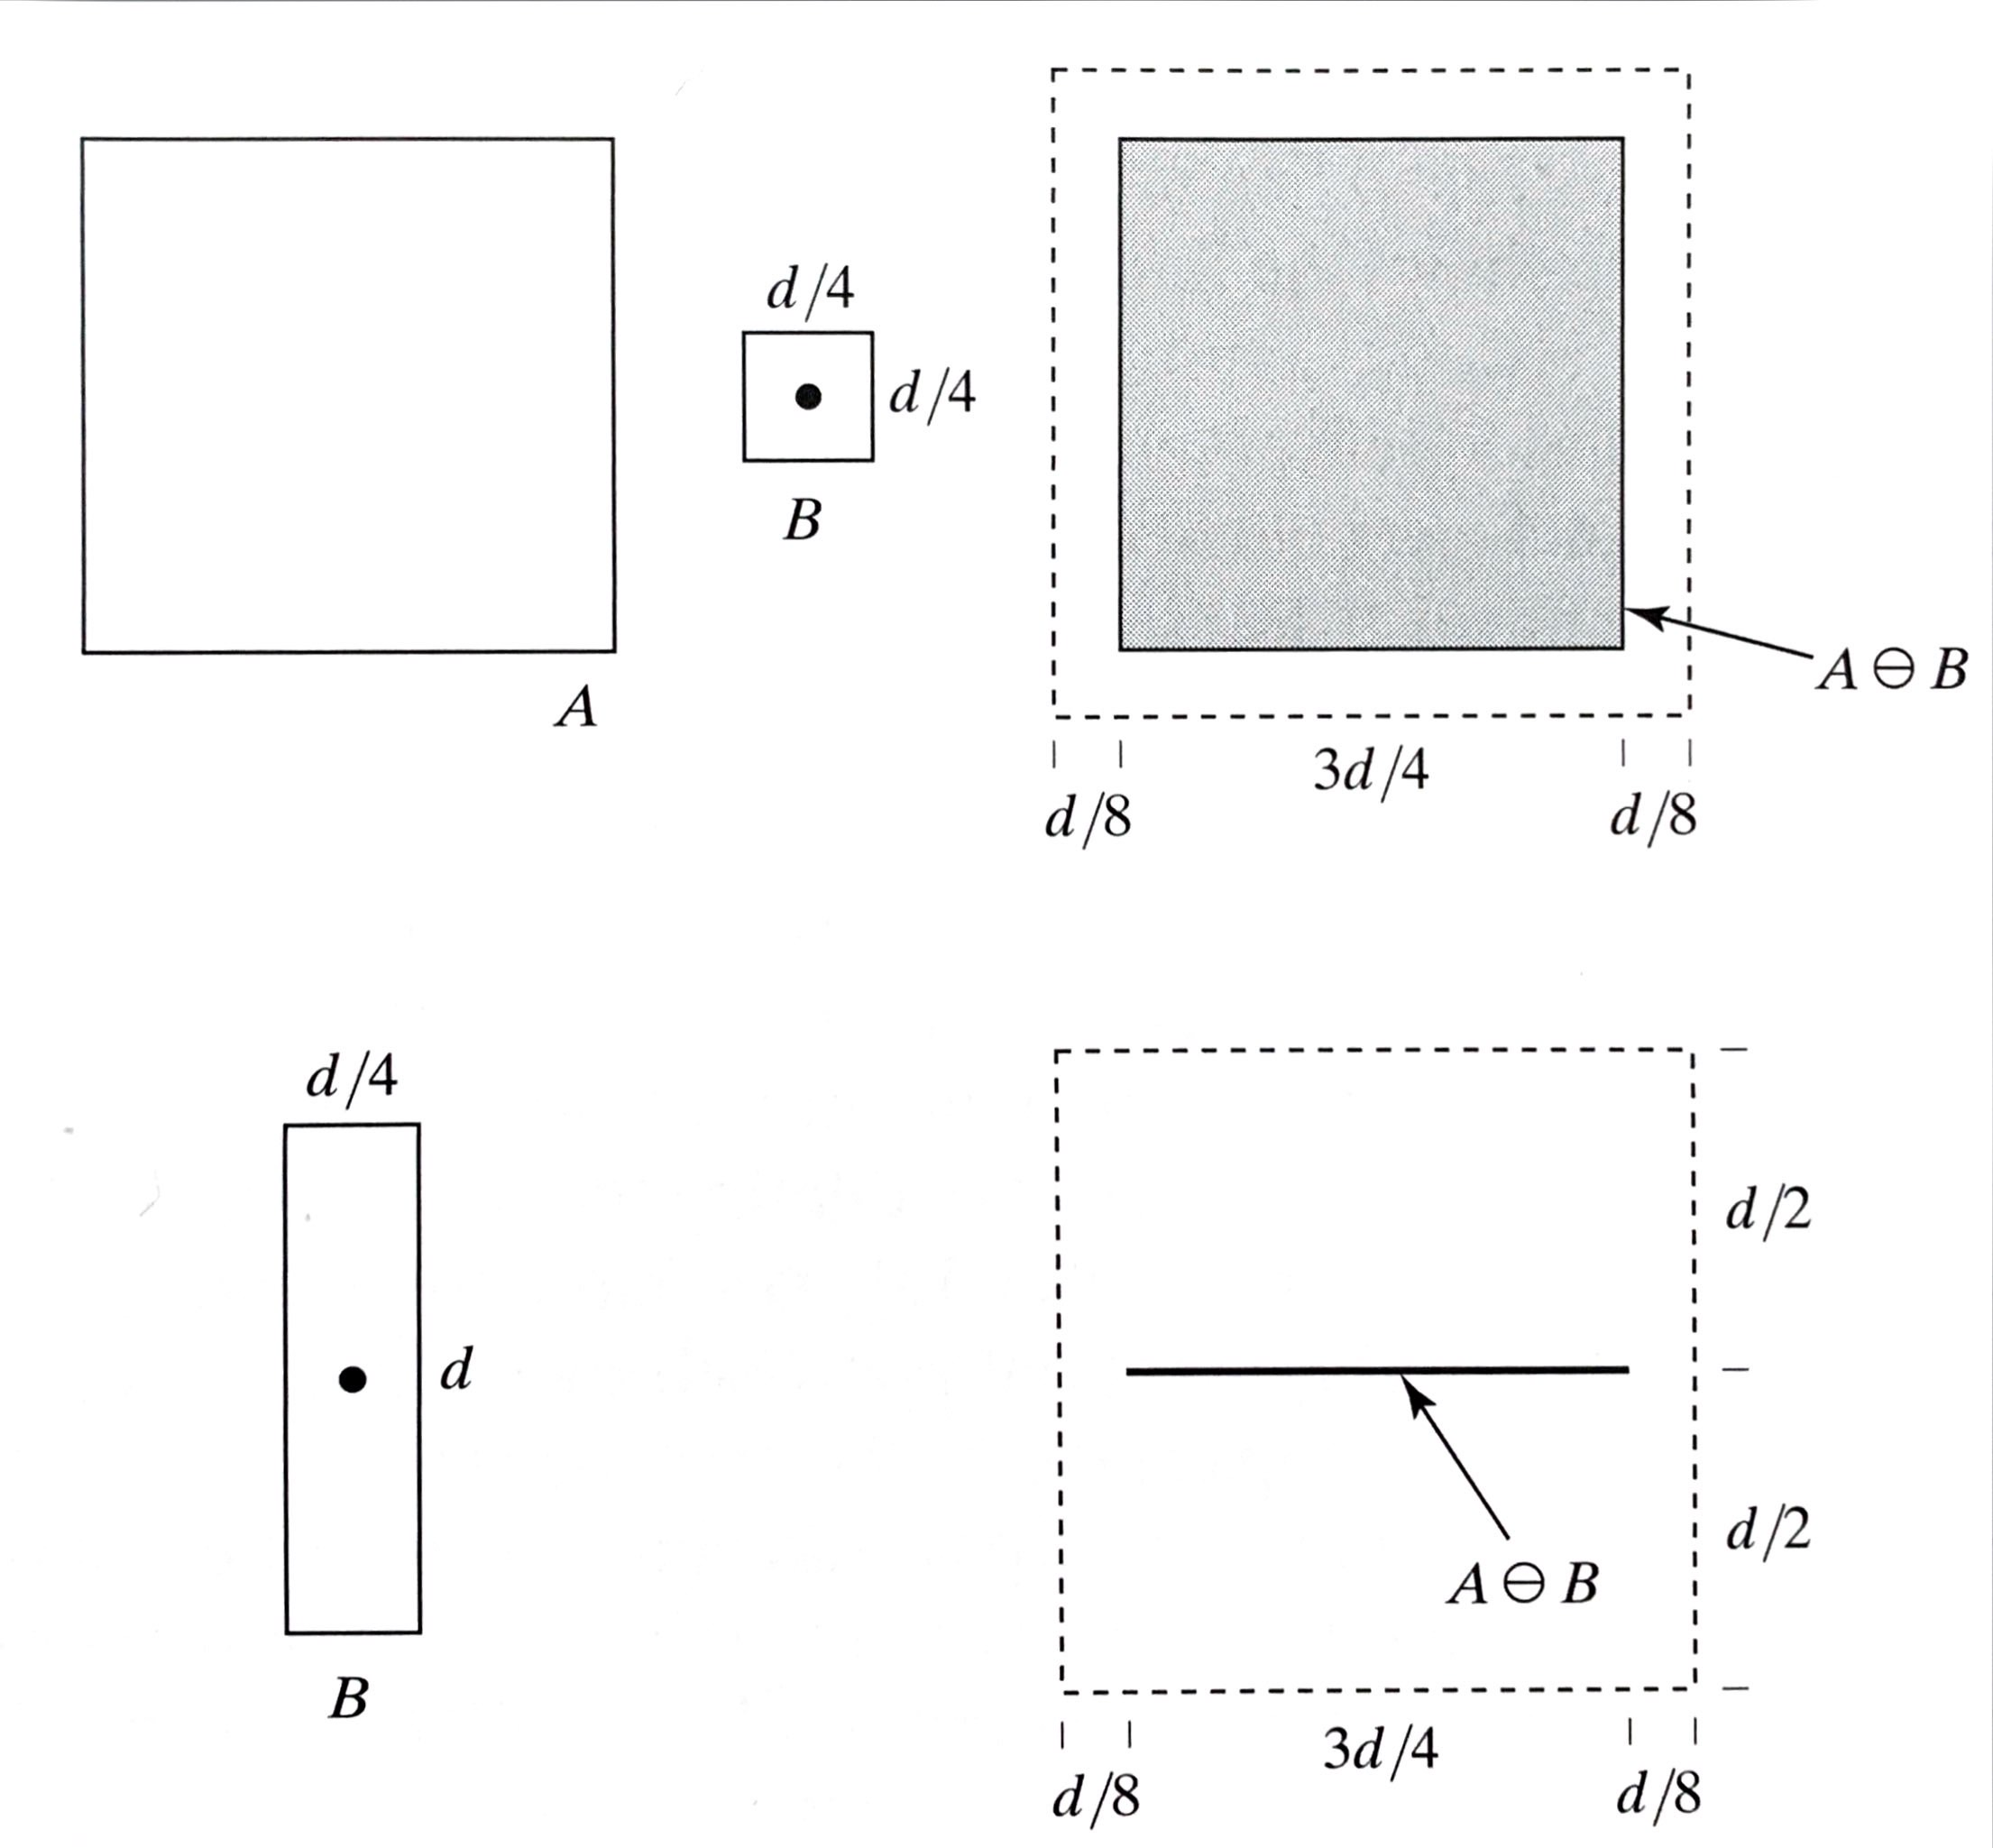
\includegraphics[width=6.3cm]{resources/morph_erosion.jpg}
    \end{center}
    \caption{Morphological erosion (Gonzalez 2002)} % todo: Replace
    \label{fig:morph_erosion}
\end{figure}

\subsection{Opening and closing}

Now that the basic two operations have been defined, we can move on to two
very useful operators, morphological opening and morphological closing.

\subsubsection{Opening}

The morphological opening is defined as erosion followed by a dilation with a
reflected structural element, formally the opening $\circ$ of a set $A$ by a structuring
element $B$ is defined as\cite{soile2004}: 

$$A \circ B = (A \ominus B) \oplus \hat{B} $$

This process in visualised in Figure \ref{fig:opening}, where the square
structural element is applied on the binary image. Morphological opening
preserves larger structural components, and removes small objects from the
image. This means, it is a good candidate for removing noise, small objects or
thin structures, which may interfere with later processing.

\begin{figure}
    \begin{subfigure}[t]{0.4\textwidth}
        \centering
        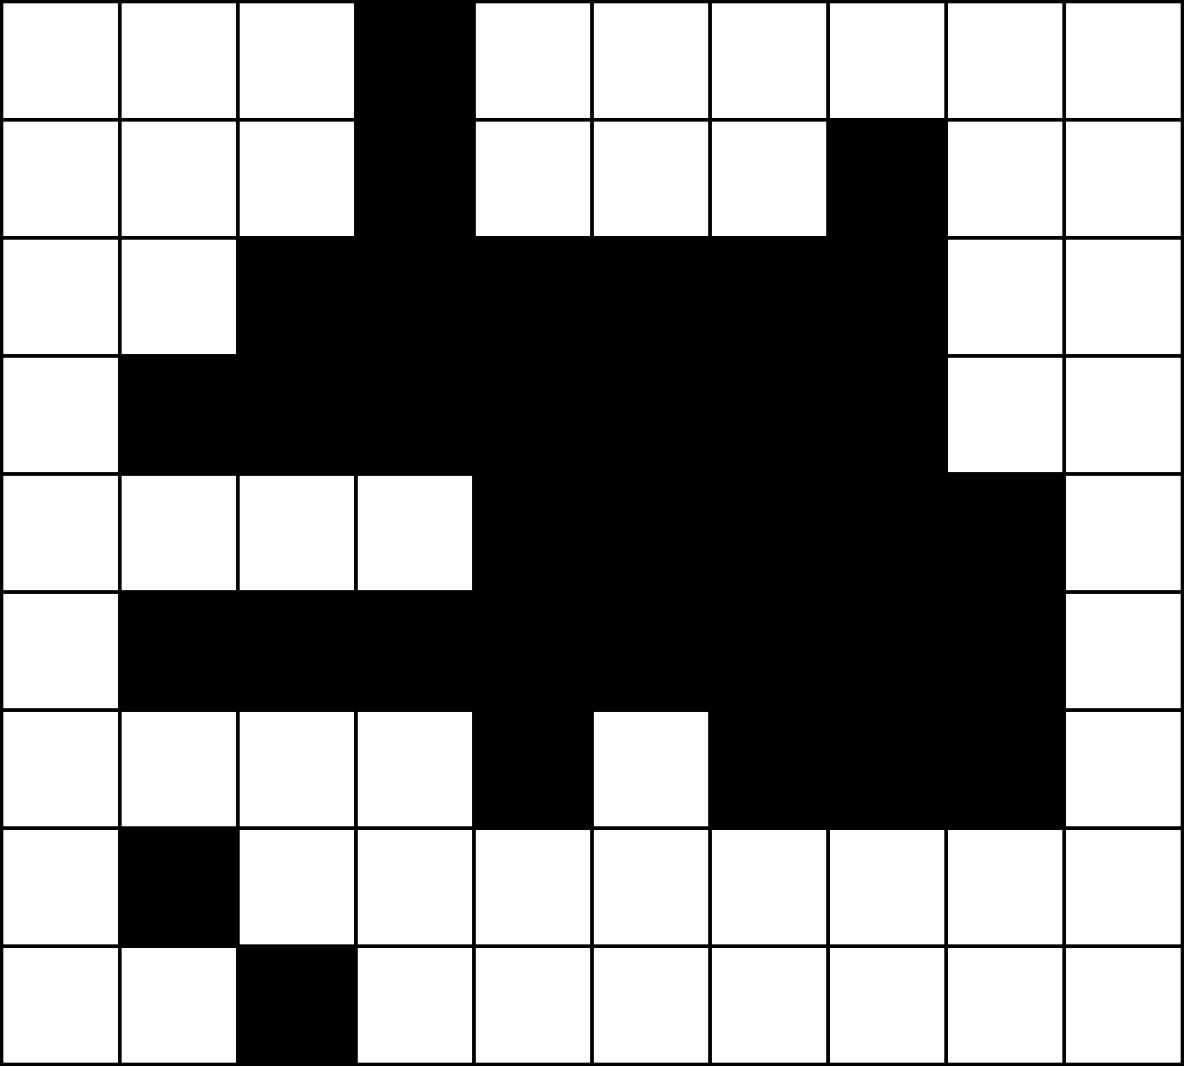
\includegraphics[width=\textwidth]{resources/inkscape/opening_orig.png}
        \caption{A binary image A.}
        \label{fig:opening_orig}
    \end{subfigure}
    \begin{subfigure}[t]{0.4\textwidth}
        \centering
        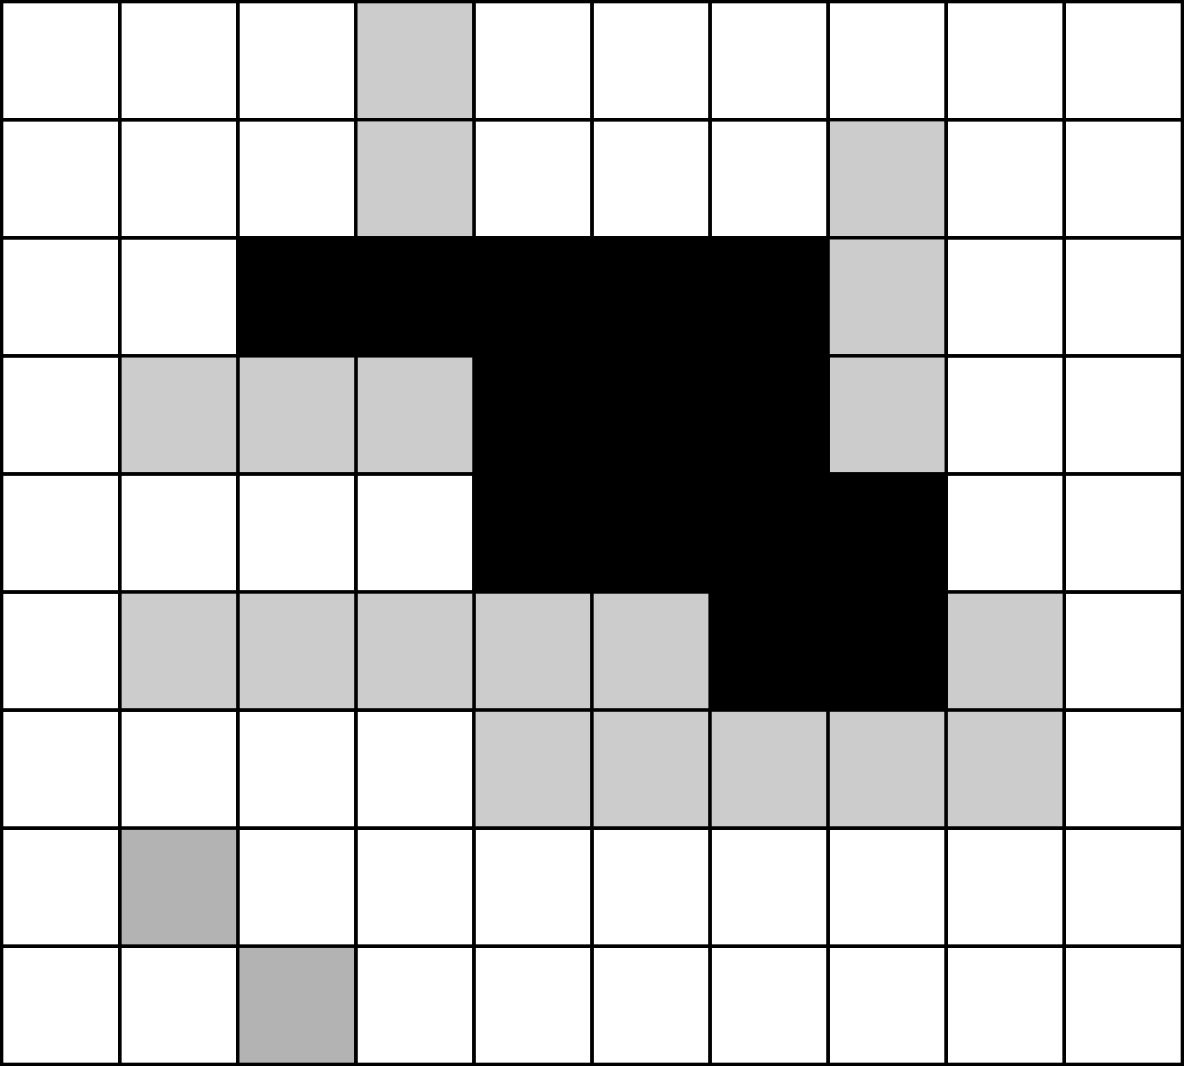
\includegraphics[width=\textwidth]{resources/inkscape/opening_erosion.png}
        \caption{Erosion of image A.}
        \label{fig:opening_erosion}
    \end{subfigure}
    \begin{subfigure}[t]{0.2\textwidth}
        \centering
        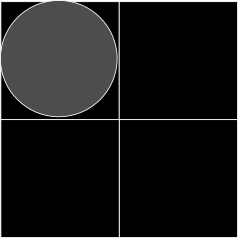
\includegraphics[width=\textwidth]{resources/inkscape/opening_erosion_se.png}
        \caption{Structural element used in erosion.}
        \label{fig:opening_erosion_se}
    \end{subfigure}
    \begin{subfigure}[t]{0.4\textwidth}
        \centering
        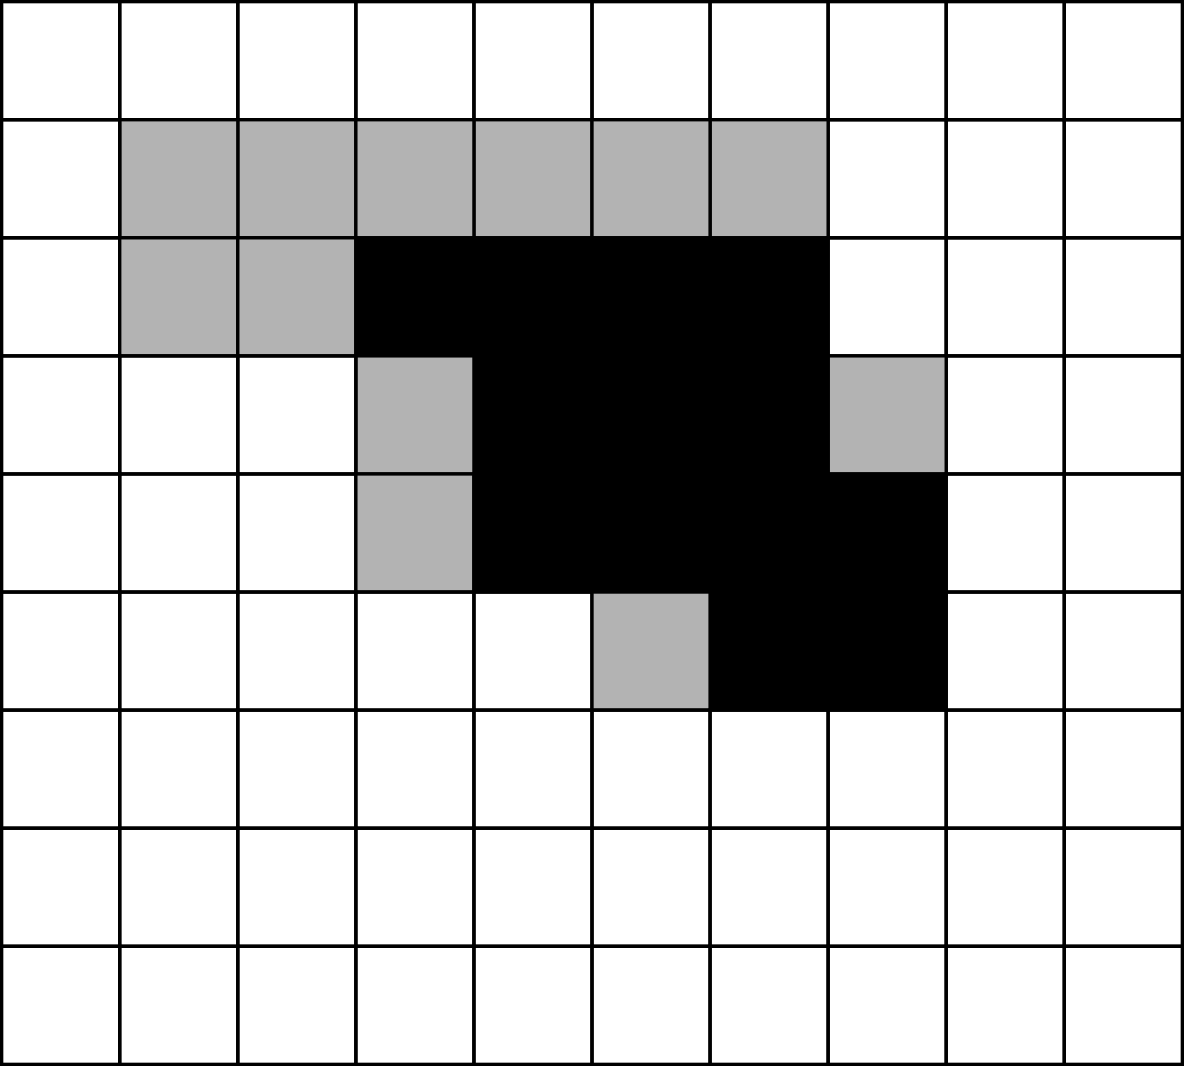
\includegraphics[width=\textwidth]{resources/inkscape/opening_dilation.png}
        \caption{Dilation after erosion of image A.}
        \label{fig:opening_dilation}
    \end{subfigure}
    \begin{subfigure}[t]{0.2\textwidth}
        \centering
        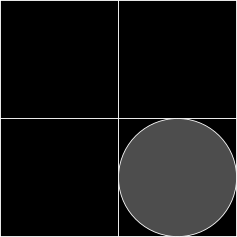
\includegraphics[width=\textwidth]{resources/inkscape/opening_dilation_se.png}
        \caption{Structural element used in dilation.}
        \label{fig:closing_dilation_se}
    \end{subfigure}
    \caption{Morphological opening of the image A. Centres of structural
    elements are indicated by the circles. The gray pixels indicate which pixels
    were lost (erosion) or added (dilation) after the transformation.}
    \label{fig:opening}
\end{figure}

\subsubsection{Closing}

The morphological closing is defined similarly to the opening, but the order of
operations is reversed. The closing $\bullet$ of a set $A$ by a structuring
element $B$ is defined as\cite{soile2004}: 

$$A \bullet B = (A \oplus B) \ominus \hat{B} $$

\begin{figure}
    \begin{subfigure}[t]{0.4\textwidth}
        \centering
        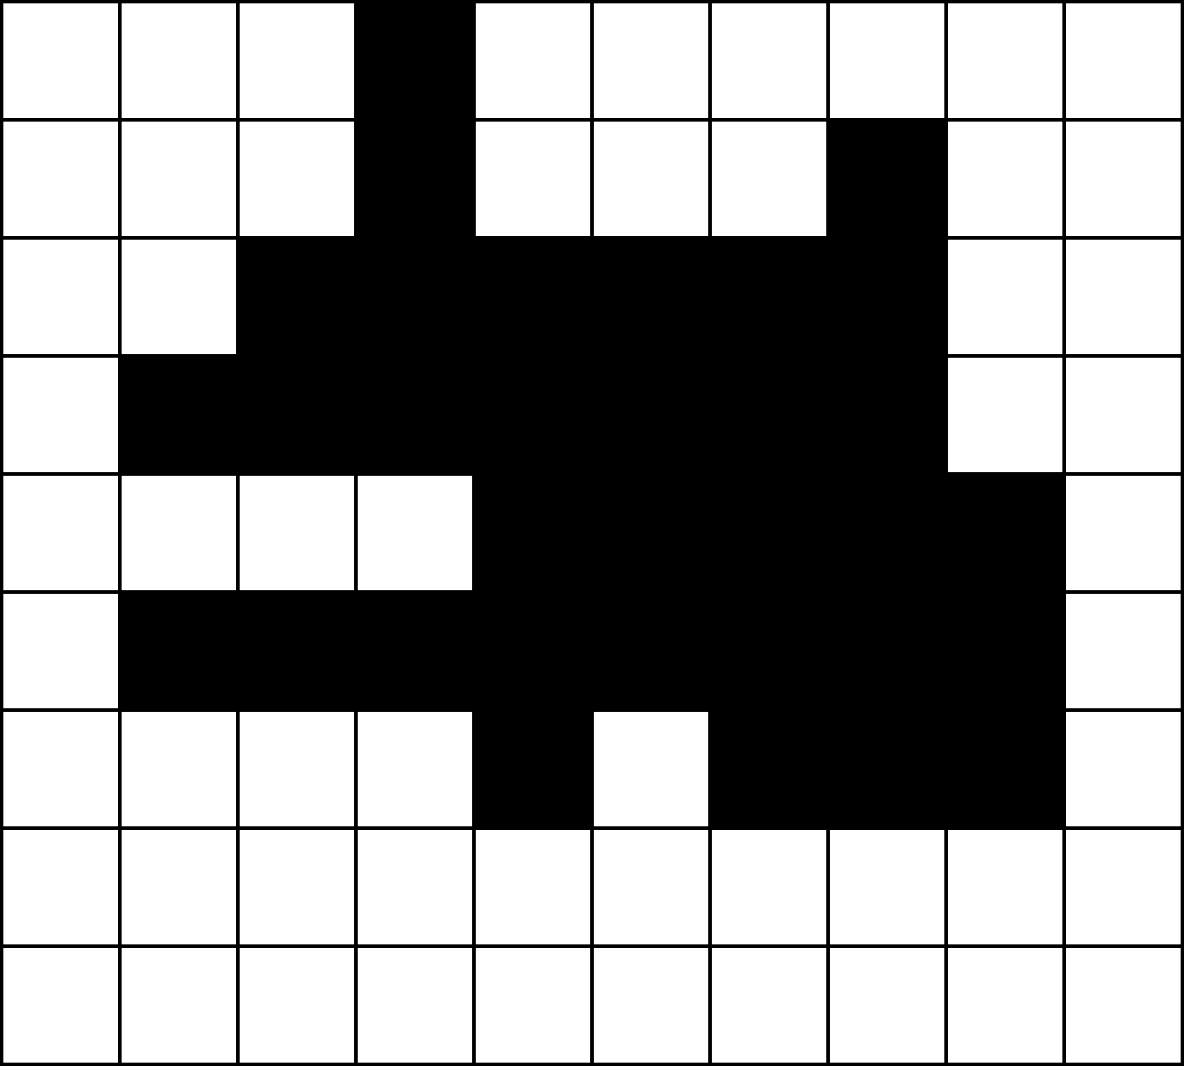
\includegraphics[width=\textwidth]{resources/inkscape/closing_orig.png}
        \caption{A binary image A.}
        \label{fig:closing_orig}
    \end{subfigure}
    \begin{subfigure}[t]{0.4\textwidth}
        \centering
        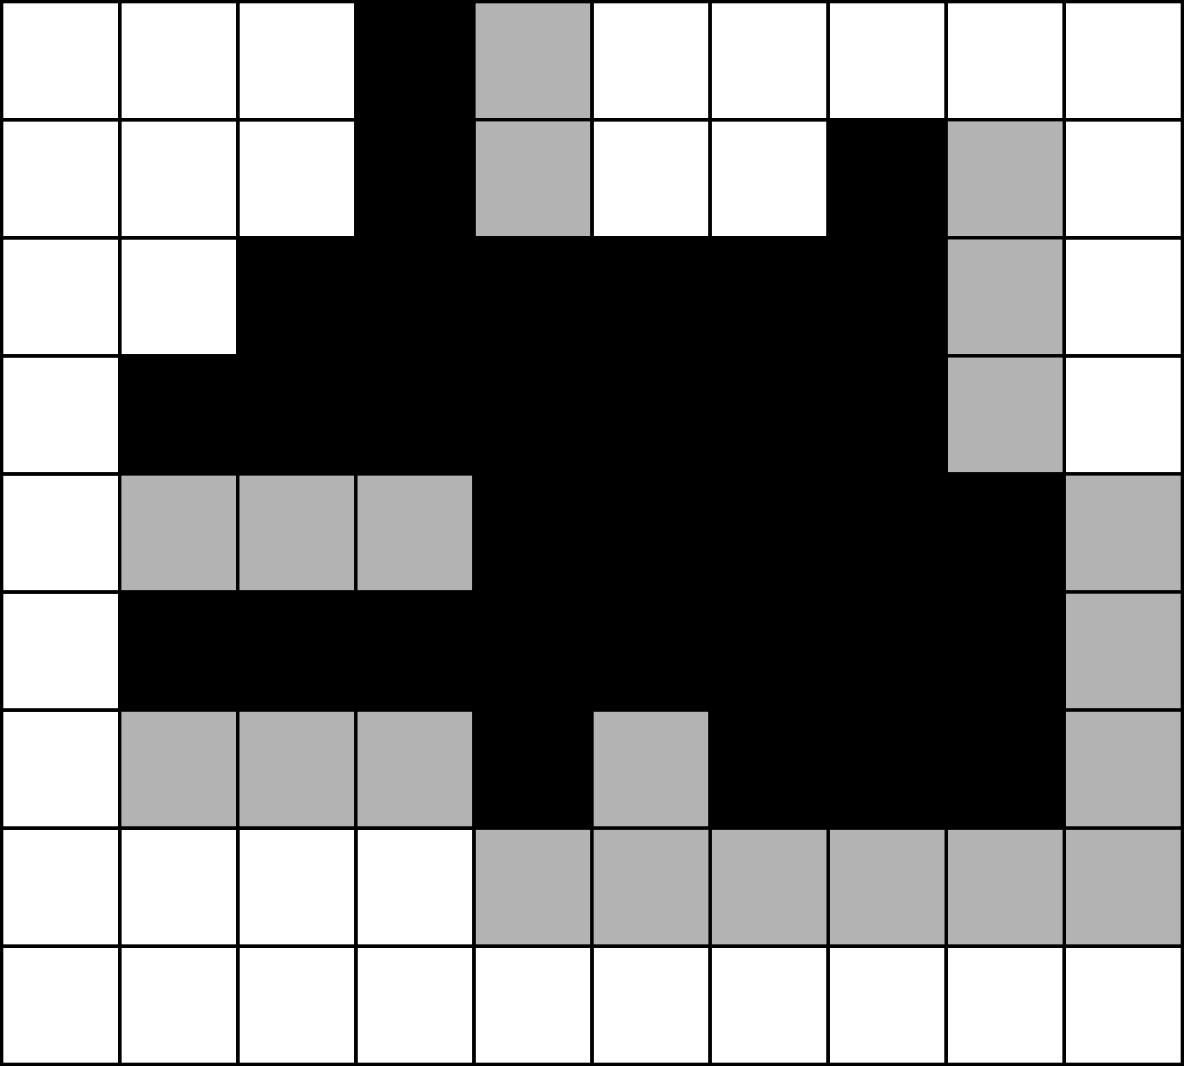
\includegraphics[width=\textwidth]{resources/inkscape/closing_dilation.png}
        \caption{Dilation of image A.}
        \label{fig:opening_erosion}
    \end{subfigure}
    \begin{subfigure}[t]{0.2\textwidth}
        \centering
        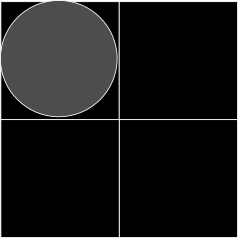
\includegraphics[width=\textwidth]{resources/inkscape/opening_erosion_se.png}
        \caption{Structural element used in dilation.}
        \label{fig:opening_erosion_se}
    \end{subfigure}
    \begin{subfigure}[t]{0.4\textwidth}
        \centering
        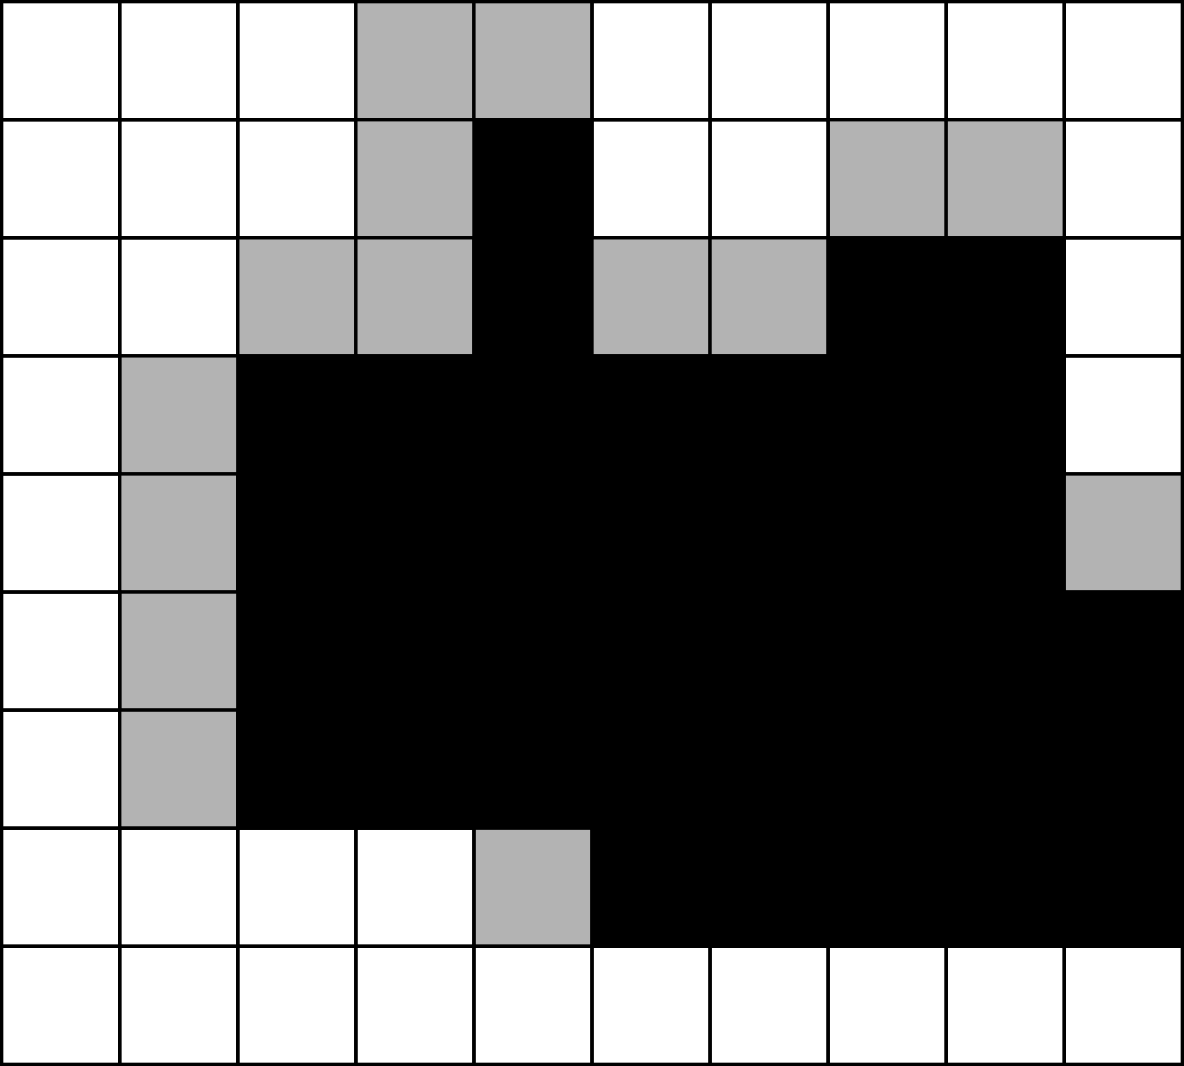
\includegraphics[width=\textwidth]{resources/inkscape/closing_erosion.png}
        \caption{Erosion after dilation of image A.}
        \label{fig:opening_dilation}
    \end{subfigure}
    \begin{subfigure}[t]{0.2\textwidth}
        \centering
        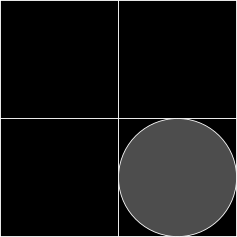
\includegraphics[width=\textwidth]{resources/inkscape/opening_dilation_se.png}
        \caption{Structural element used in erosion.}
        \label{fig:closing_dilation_se}
    \end{subfigure}
    \caption{Morphological closing of the image A. Centres of structural
    elements are indicated by the circles. The grey pixels indicate which pixels
    were lost (erosion) or added (dilation) after the transformation.}
    \label{fig:closing}
\end{figure}

Like for the previous operator, this is visualised in Figure \ref{fig:closing},
where the square structural element is applied on the binary image. 
Morphological closing, like the opening, keeps the larger structural elements,
but also fills in holes, which might have been created for example by noise.
Also, it does not remove small objects.

While mathematical morphology is a massive topic of interest to many
researchers, here I will only use the aforementioned operations. They can be
further used to define more operations such as performing top hat transforms,
skeletonizing images, finding perimeters etc \cite{mathworks_morp_oper}.

\section{Segmentation}

\textbf{TODO}

\subsection{Watershed algorithm}

The watershed algorithm is a wide-spread technique for image segmentation. The
fundamental principle of the watershed algorithm is to view the image as a
topological map, where the intensities indicate the height of the landscape, in
other words, peaks in the image represent mountains or hills while low values
represent valleys.

The algorithm then creates water springs at these valleys, from which the water
flows at a uniform rate. As the waters from different springs rises, they might
start to mix. At these points we build dams to separate the various flooded
areas. The water continues to flow until just the dams are visible above the
water \cite{gonzalez2002}. At this point the image is segmented using the dams,
and every catchment basins is uniquely labelled.

\textbf{TODO: Copy image from textbook}
\textbf{TODO: Consider explaining markers are water sources here or in later
chapters.}

\chapter{Image data}

The image data --- of mouse mammary organoids --- was acquired using confocal
laser scanning. The original data was captured in 2021 by a group of
researchers at (\textbf{TODO}) faculty. The captured specimen is around 500
microns by 500 microns by 80 microns, and a single voxel's size is $0.233\mu m$ by
$0.233\mu m$ by $0.586\mu m$.

In confocal scanning, researchers are able to stain specific structures in
their specimen so that wanted structures reemit light when the proper wavelength
is shined upon them. This allows them to capture the density of studied proteins
inside the specimen. In this particular case, the researchers captured the
density of 3 different proteins, of which one is part of membranes, while the
other two are primarily located inside the cell's nuclei.

The data, totalling around 576 GB, consists of 12 different time steps, where
each step has a size of 1920x1920x388 pixels. For every protein, the researchers
captured the image using two different optical setups; thus, there are six
channels. The data is stored in numerous TIFF files, and every channel contains
grayscale data with 16 bits per pixel. 
\begin{figure}
    \begin{subfigure}[t]{0.4\textwidth}
        \centering
        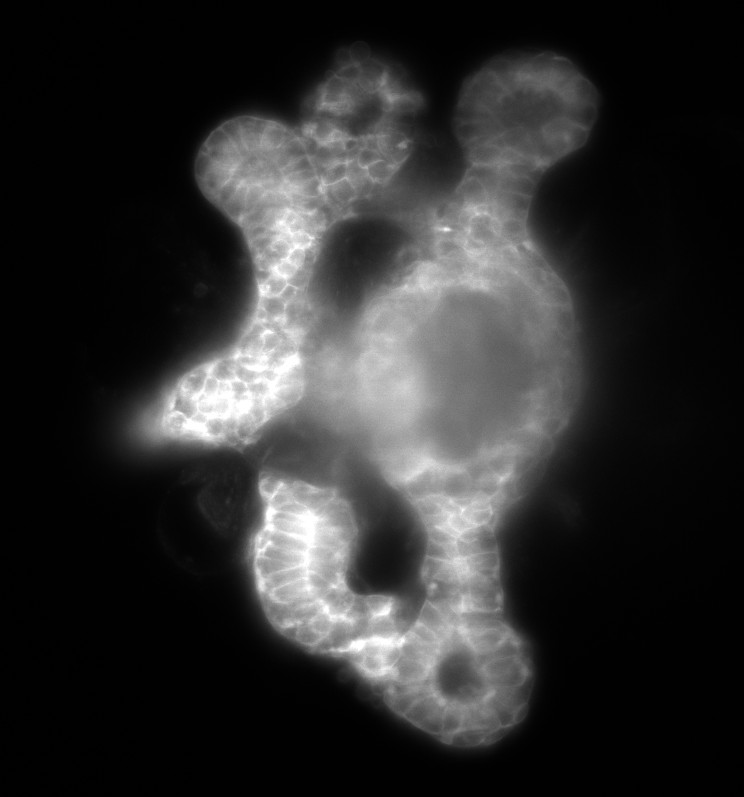
\includegraphics[width=\textwidth]{resources/C3-t006-200-scaled.jpg}
        \caption{Membrane-stained channel.}
        \label{fig:data_example_membraine}
    \end{subfigure}
    \begin{subfigure}[t]{0.4\textwidth}
        \centering
        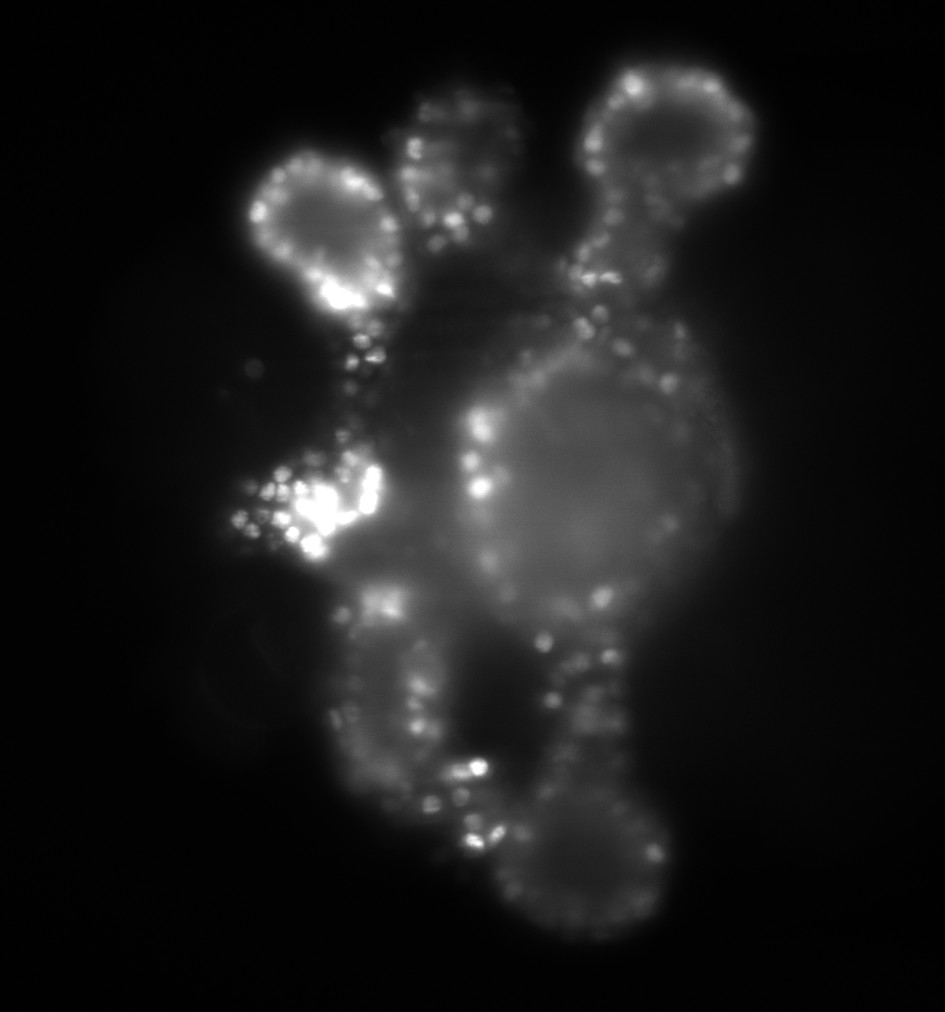
\includegraphics[width=\textwidth]{resources/C2-t006-200-scaled.jpg}
        \caption{Nuclei-stained channel.}
        \label{fig:data_example_nuclei}
    \end{subfigure}
    \caption{A sample from the data.}
    \label{fig:data_example}
\end{figure}
In the Figure \ref{fig:data_example} a single slice of the data was taken from
two channels. They are from the same time point and from the same place.

\section{Problems with the dataset}

The size of the data and the inherent problems of fluorescence microscopy
provide the main issues in analysing the data. It is very time consuming to
analyse the whole data set; therefore, all work was done on much smaller slices
of the data. Interesting regions with well lit

\begin{figure}
    \centering
    \begin{subfigure}[t]{0.5\textwidth}
        \centering
        \frame{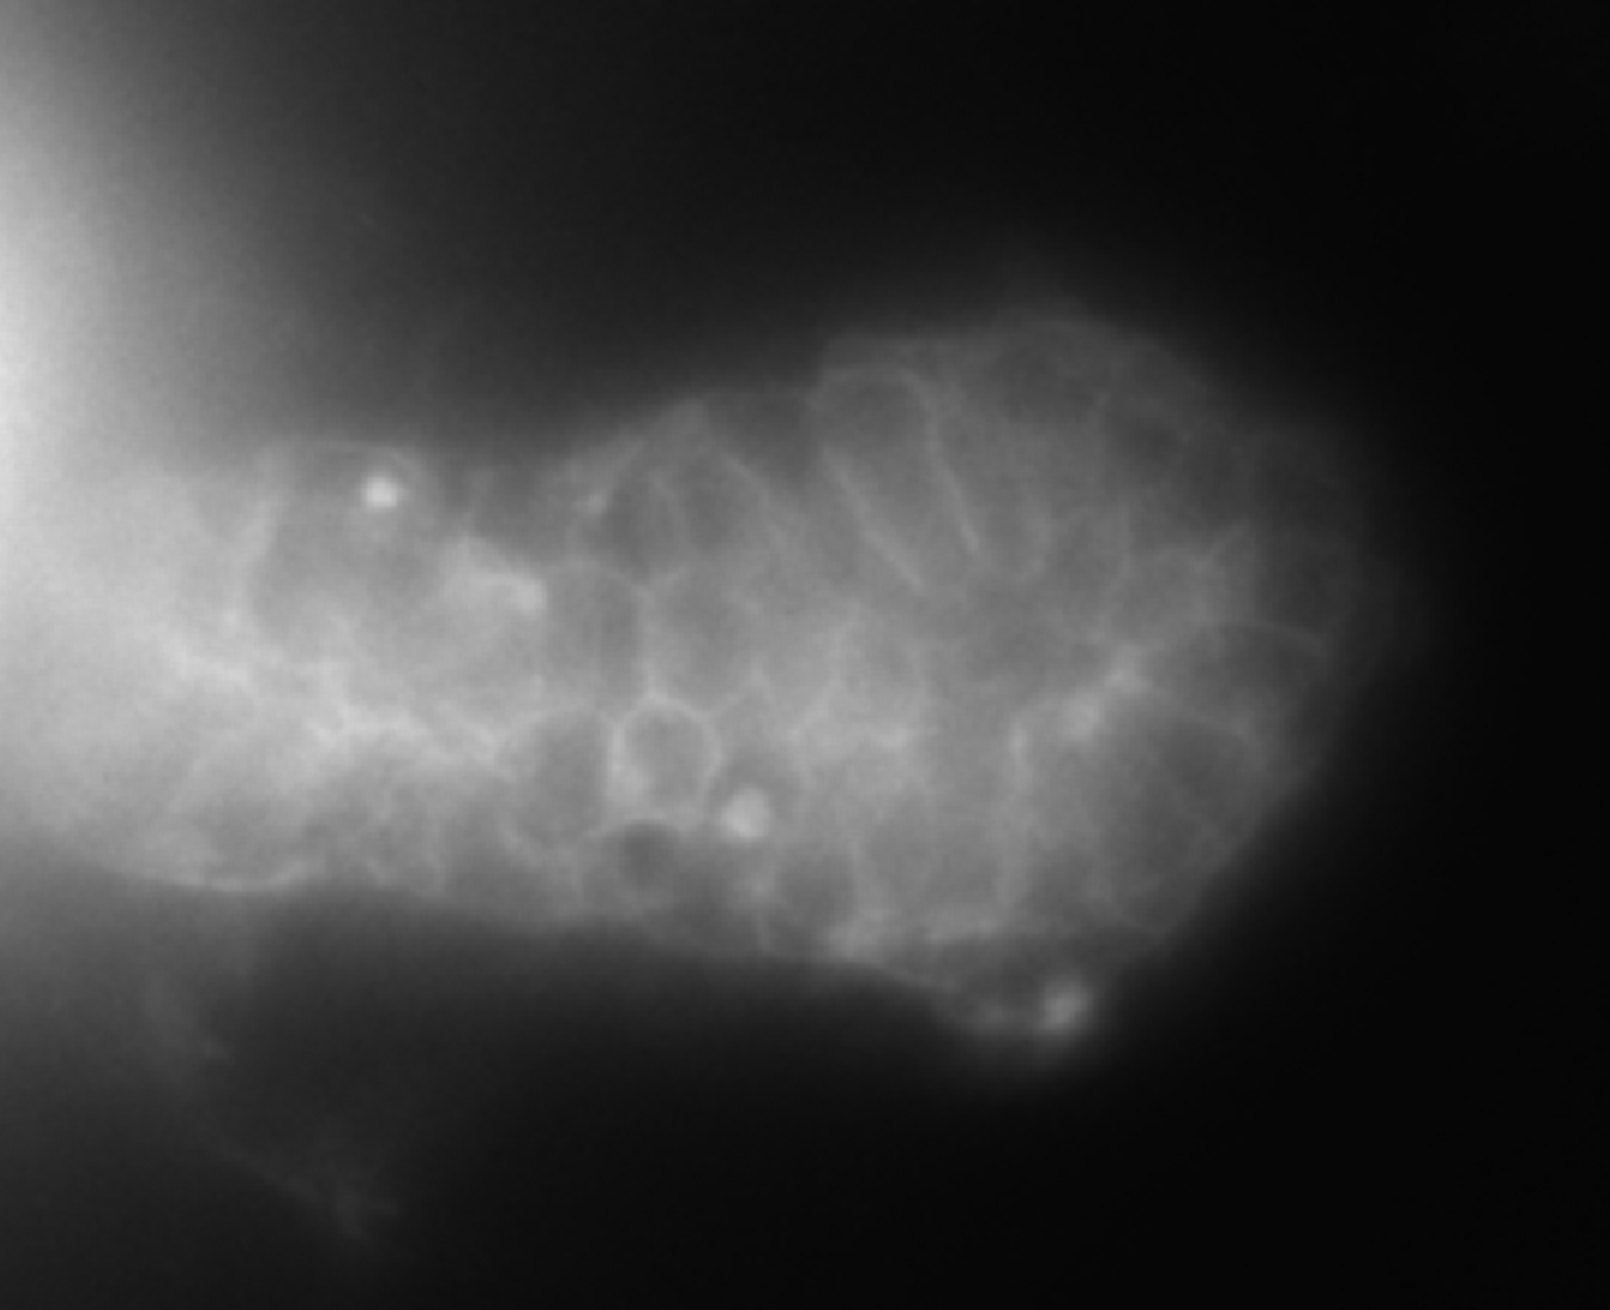
\includegraphics[width=\textwidth]{./resources/bad-edges.png}}
        \caption{In this image, many of the inner edges are missing.}
        \label{fig:bad_edges}
    \end{subfigure}
    \hfill
    \begin{subfigure}[t]{0.3\textwidth}
        \centering
        \frame{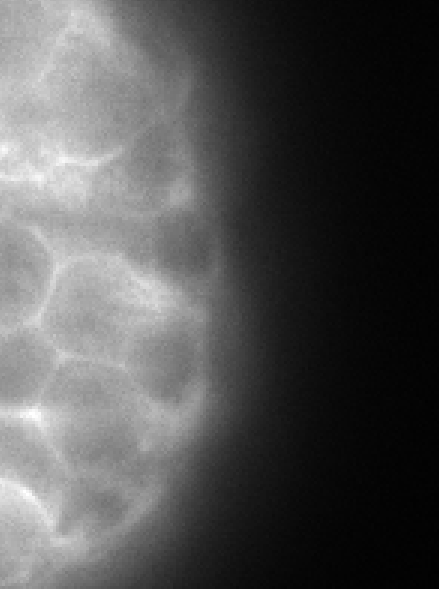
\includegraphics[width=\textwidth]{./resources/bleading-edge.png}}
        \caption{Here, there is not a clear edge between the inner cell and the
        background.}
        \label{fig:bleeding_edges}
    \end{subfigure}
    \hfill
    \begin{subfigure}[t]{0.5\textwidth}
        \centering
        \frame{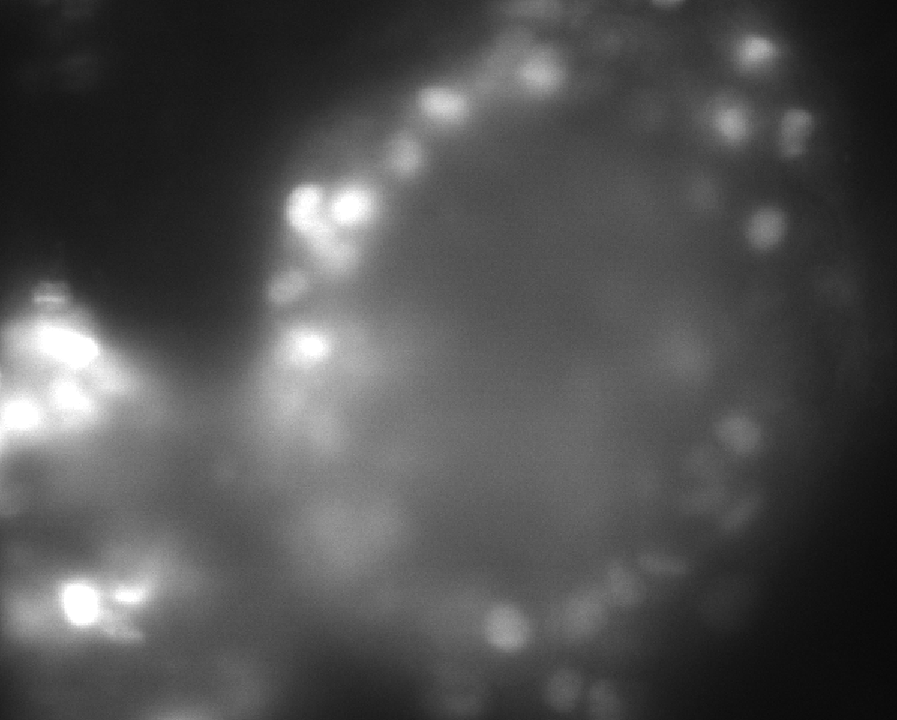
\includegraphics[width=\textwidth]{./resources/light-scattering.png}}
        \caption{Scattering inside the cell, causing large problems with the
        segmentation.}
        \label{fig:scattering}
    \end{subfigure}
    \caption{Typical issues with the data.}
    \label{fig:labelling_example}
\end{figure}

\subsection{Noise}

The first problem with the data set is the quality. In most places, the noise is
too strong to try to use it in any analysis.

In the membrane channel, two main problems can be seen seen. To begin, most
membranes do not form connected segments, instead, a part the cell's membrane is
usually missing or it is joined with the neighbouring cell's membrane as can be
seen in Figure \textbf{\ref{fig:bad_edges}}. This complicates the analysis, as different
regions may require different filters to be properly preprocessed. Moreover,
this makes the edge detection much harder, since it relies on the magnitude of
gradient of the image. Moreover, sometimes the gradient between the cell and the
background is too smooth for the program to found the divisive line as in Figure
\ref{fig:bleeding_edges}.

Another issue is that the light gets scattered inside the organoid as can be seen
in Figure \textbf{\ref{fig:scattering}}. That means that it is possible to analyse only the
outer most layers of cells of the organoid.

The protein channel comes with its own set of problems, some of them different.
It is still true, that the sharpest data comes, again, from the outermost layer
of the organoid, limiting the amount of usable data. Another issue is that the
individual cells are sometimes quite fuzzy, which makes it hard to decide, where
exactly the cells ends, or if they are multiple cells.
% todo: reword

\subsection{Size}

The size of the dataset poses the second problem, as it would be computationally
expensive to try to process the whole data set at once; however a lot of the
data is either unusable or of no interest. In most instances, the data is
predominantly composed of the background, and at several moments in time, no
specimen can be seen; therefore, to reduce the computational demands further,
only specific regions of interest were manually selected to create the final
data set. In the end, the reduced data set is only a few dozen megabytes large.

\section{Dataset}

For reasons specified in the previous sections it would not be reasonable
to run the evaluation algorithm on the whole dataset. Moreover, it is not clear,
how prediction on the whole dataset would be scored, not to mention the large
computing and storage requirements; thus, we decided to create a set of images
on which the algorithm will be evaluated. The set contains 11 images, which I
hand picked from the raw data. I tried to include sections from various
channels, times, and in variety of the quality. This was done to test the
program's performance and precision under variety of different circumstances.


All of the images are included as attachments in the thesis. The general
namescheme is \texttt{txxx-roi-y-z}, where \texttt{xxx} stands for the time,
\texttt{roi-y} stands for region of interest with index \texttt{y}, and the
\texttt{z} stands for the central frame. As the program is capable of using
multiple frames from the membrane-stained channel, it is possible to provide
several slices in a single image. The program then runs the maximum projection
in 3D, but the slice in the middle will be picked for further processing. On the
other hand, the nuclei-stained data is always two-dimensional.

This dataset was then passed to researchers at the faculty of \textbf{TODO} for
evaluation. They manually labelled the nuclei-stained data in the following
structure: Parts that were considered to be background was labelled using $0$.
Sections which were too complicated or unclear were labelled using $65535$, and
the rest of the cells were uniquely labelled with numbers starting at $1$. In
Figure \ref{fig:label_ground_truth} the segmentation created by the expert of
the \ref{fig:label_membrane_channel} is shown.

\begin{figure}
    \centering
    \begin{subfigure}[t]{0.4\textwidth}
        \centering
        \frame{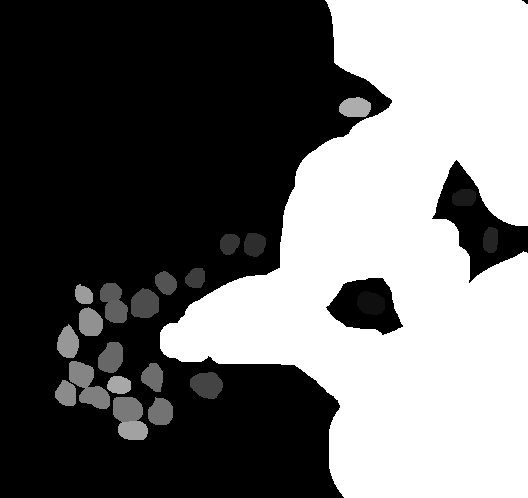
\includegraphics[width=\textwidth]{./resources/ground-truth.png}}
        \caption{Ground truth labelling created by an expert. White means
        complicated area, black is background, the rest are cells.}
        \label{fig:label_ground_truth}
    \end{subfigure}
    \hfill
    \begin{subfigure}[t]{0.4\textwidth}
        \centering
        \frame{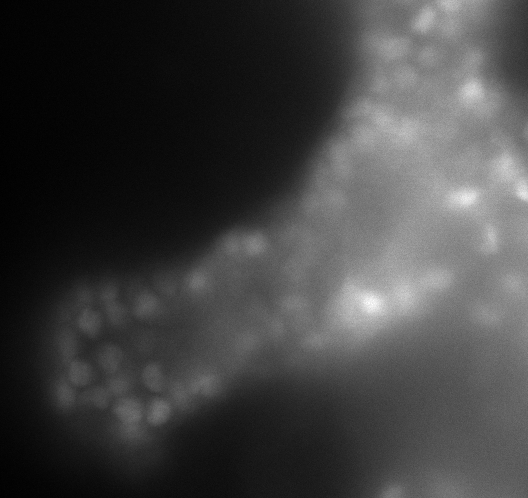
\includegraphics[width=\textwidth]{./resources/membrane-channel.png}}
        \caption{Image from membrane-stained channel.}
        \label{fig:label_membrane_channel}
    \end{subfigure}
    \hfill
    \caption{Expert's labelling of the image on the right.}
    \label{fig:labelling_example}
\end{figure}


\chapter{The developed segmentation method}

%todo: inkorporovat fakt, ze hlavne v jadrovom kanale to robime
%note: Overview/Goals;High level overview of the process.

The goal of the algorithm is to segment individual cells and uniquely label each
cell; however, as previously discussed, they are often not clearly separated
from each other. A naive Otsu thresholding leads to NEUSPOKOJIVE results as is
seen on Figure \textbf{TODO}. Thus, a more sophisticated algorithm had to be
developed to segment the cells' nuclei finer.

We settled on two step algorithm. In the first step, the membrane-stained
channel is used, while in the second step the nuclei-stained channel is used.
Every cell has a membrane and a nuclei in our specimen; hence, we should be able
to use the information provided by the first channel to improve the thresholding
in the second channel.

In the first step quite DRSNA segmentation is performed to roughly find the
membranes separating the individual cells. The segmentation is then utilized in
the second step; the algorithm overlays the previous segmentation on top of the
protein-stained channel and looks at every label. Each one represents a single
cell, and some of it's surroundings. Finally, a local version of the gradient 
threshold is performed on each region.

\begin{figure}
    \begin{center}
        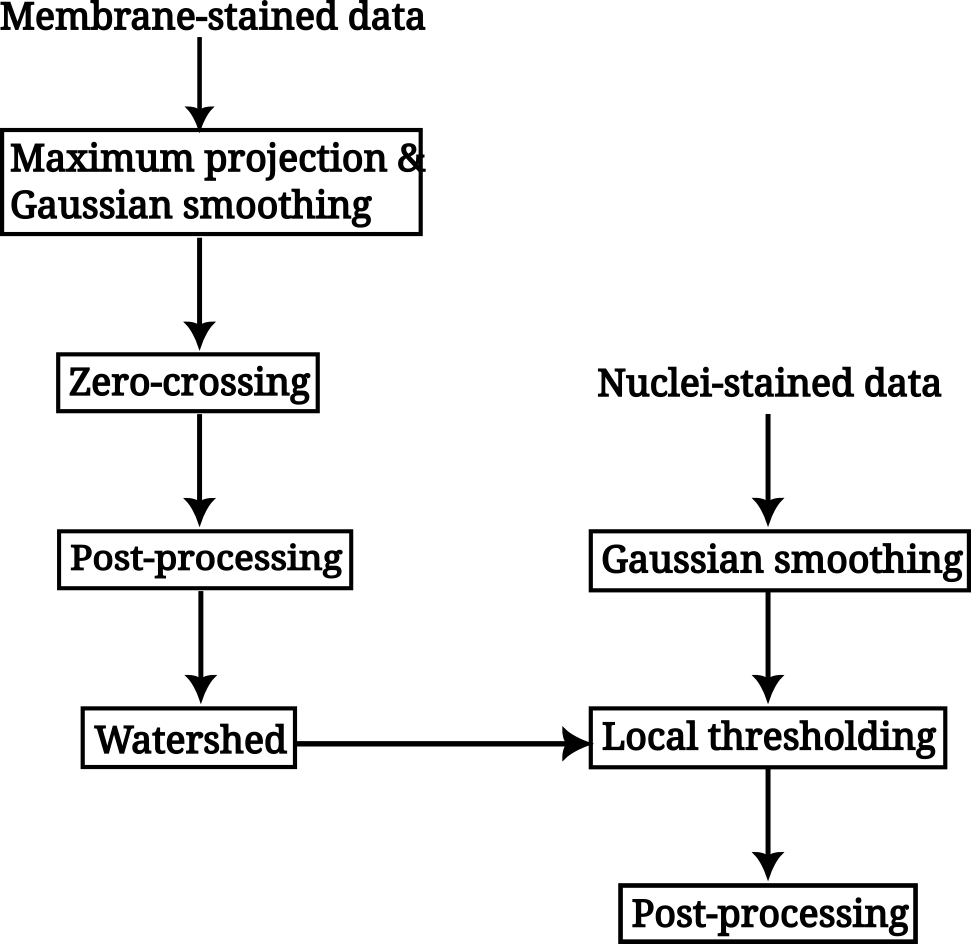
\includegraphics[width=10cm]{./resources/inkscape/segmentation-steps.png}
    \end{center}
    \caption{All steps in the segmentation algorithm.}
    \label{fig:segmentation_steps}
\end{figure}

\section{Membrane channel}
Steps inside the membrane channel: watershed, thresholding, denoising, edge
detection

The goal is to provide a rough segmentation of the cells using the
membrane-stained channel. First, a pre-process of the data is performed to deal
with some of the noise in the data. As can be seen on Figure \textbf{TODO} we
need to deal with the fact, that the intensity inside the cell is quite uneven.
To even out the lighting inside cells a maximum projection from gaussian pyramid
is performed. The idea behind this step is, that edge have higher intensities
than insides of the cells; therefore they should not be very influenced by this
step. At the same time the uneven lighting inside cells will be smooth out,
since the highest intensity areas will \textbf{bleed} out to the surrounding
area. This effect is demonstrated on the Figure \textbf{TODO}. That concludes
the denoising part.

% TODO: rephrase this
Naively applying the zero-crossing algorithm results in other artefacts, such
as noise causing the algorithm to find contours in the background; therefore,
a cell mask must be created to differentiate between the foreground (the
specimen) and the background. For this task, the Otsu thresholding method was
used, due to a bimodal distribution of the data \textbf{TODO}. On the Figure
\textbf{TODO} the thresholded data along with the histogram is shown. However,
some of the useful data is incorrectly labelled as background, to combat this, in
a general form a binary erosion with a circular structural element with radius
equal to user-defined cell radius. The final version is show in the second row
in Figure \textbf{TODO}.

After dealing with the uneven lighting the edge detection is performed. To help
with the residual noise, anisotropic Gaussian smoothing is applied. The voxel
dimensions in our data is not the same as in the z-axis the voxel is about 2.5
times as large; hence, using an anisotropic filter is more correct. 

Now the pre-processing is finished and the zero-crossing algorithm is applied.
The zero-crossing algorithm provides a reasonable outline of the cells as is
shown in Figure \textbf{TODO}. The user sometimes has to play around with
various sigmas to improve the quality of the edge detection. When the sigma is
too low the algorithm tends to find a large amount of small regions, while too
large sigma causes the algorithm to join individual cells together. This step
is further complicated by the fact, that some of the cells are missing parts of
their membranes. \textbf{TODO}; hence, the is one of the limiting factors of
the segmentation pipeline.

Next step is to utilize the outlines to segment individual cells. For this task
the watershed algorithm is used. To improve the quality of the segmentation,
markers indicating the sources of water need to be created. Ideally, every cell
has one marker. These markers are then fed to the watershed algorithm as places
from which water stems from. %TODO tu som vymazal cast 
The distance map and the markers are then passed to the
watershed algorithm. It labels each cell with a unique label.

A great advantage of creating the markers from the distance map is that, even if
the edge detections joins several cells together, the two cells can still be
labelled individually.

\section{Nuclei-stained channel}

Steps inside the protein channel: thresholding, denoising

In Figure \textbf{TODO} a common example of the nuclei-stained channel is shown.
In this channel the preprocessing consists of just a simple Gaussian smoothing
to help with the thresholding.

Applying the Otsu thresholding method in the nuclei-stained channel leads to
poor results as is seen in Figue \textbf{TODO}. The problem is that the lighting
is quite uneven. Some cells are significantly brighter than others; thus, global
thresholding is not a viable option.

However, we can use the previously obtained segmentation from membrane-stained
channel to improve the quality of the thresholding. By looking at just specific
areas denoted by the labels, the thresholding yields more suitable results. In
essence, a local version of some thresholding algorithm can be used.

In our testing, Otsu thresholding method was not suitable as in many cases the
proximity of cells shrinks the background area, causing the algorithm to
categorise some of the foreground as the background. After some experimentation,
we concluded that the gradient thresholdolding algorithm provides better result.
In Figure \textbf{TODO} a comparison is made between these two algorithms. Also
others easily accessed thresholding methods in the scikit library were
experimented with, but the gradient thresholding method provided reasonable
results in many cases.

% todo: tu asi neni jasne, ze sa to robi postupne
Even tough the data was smoothed before applying the threshold, many edges in
the binary thresholded image appear quite jagged, to combat this a final round
of post-processing is applied. It consists of applying binary morphological
closing on each label to fill in dark spots; thus, rounding of the jagged edges.

An example of the final segmentation and the ground truth --- created by a
biologist --- is shown in Figure \textbf{TODO}. This concludes the section about
how the algorithm works. In Figure \textbf{TODO} several other examples of
segmentations are given.

%todo: Revise all the parameters which can be tweaked by the user.

\chapter{Implementation}
This chapter describes which libraries were used, how to run the program, and
non-trivial parts of the implementation.


\section{Justification for Python and used libraries}
As part of the bachelor thesis, I developed a terminal based program to run the
aforementioned algorithm on new data and it is available as an attachment to the
thesis. It is written in Python 3.11 and can be run after installing the
required packages. Those are specified specified inside the included
`requirements.txt` file. The environment does not need any additional setup.

I decided to use Python as my main language. Since it is an interpreted language
with dynamic typing, it allows for rapid development of new prototypes and easy
experimentation. It also has a very minimal and expressive syntax, which makes
it easy to read and write code \cite{python-docs-tutorial}. Finally, it has a
vast ecosystem of tools and libraries, which accelerates the development even
further. 

A significant disadvantage of the fact, that Python is an interpreted language,
is its, in general, poor performance. This can be mitigated to a certain degree
by using libraries instead of the default Python's data structures. Many of
these libraries use some compiled language --- such as C, C++ or Fortran --- in
the background to provide near comparable performance, while not breaking
the expressivity and simplicity of Python's syntax.

For these reasons the scientific stack based on Python was chosen instead of
other alternatives, such as the ImageJ/Fiji or OpenCV ecosystem.

The implementation heavily relies on the following packages:
\begin{itemize}
    \item{NumPy \cite{harris2020array} is an indispensable package, allowing
        Python to be utilized as a tool in scientific computing, and a
        significant part of the whole scientific computing environment in Python
        is based around this package. In its centre is the ndarray object
        representing a multi-dimensional matrix with uniform data type. The
        NumPy team has managed to utilize vectorization to greatly improve the
        performance of many common operation on matrices. This is achieved by
        writing a lot of the code in a low-level language such as C, which is
        pre-compiled and optimized, and taking advantage of the well optimized
        Intel MKL or OpenBLAS linear algebra library. This is all done in the
        background, mostly invisible to the programmer \cite{numpyManual2022}.}
    \item{SciPy \cite{2020SciPy-NMeth} provides vast set of functions and
        implemented algorithm for scientific computing. It has a wide variety of
        uses such as signal analysis, linear algebra solving, or calculating the
        Fourier transform of image. In the application this library was not used
        directly, but it is required by scikit-image.}
    \item{scikit-image \cite{scikit-image}, building on the SciPy's
        multidimensional image processing, provides numerous functions to
        process image data. The application relies on its implementation of
        Laplacian and gradient operators, mathematical morphology, and the watershed
        algorithm. As it is an extension of SciPy, it fits nicely into the
        technology stack.}
    \item{Python Imaging Library (Pillow) is a python package for reading image
        data in various formats, efficient representation of the data, and even
        some manipulating of the image data \cite{clarkc20102023}. The sole
        purpose of this packages for us, was for loading TIFF files into memory
        and storing them in a format supported by the other libraries.}
        %TODO add python standard library?
\end{itemize}
These libraries provide a great environment for writing well performing image
processing pipelines fast. All of these libraries have large communities
behind them, are continuously developed, and are open-sourced.

\section{Running the program}

The program has two main modes of operations; those are segmentation and
evaluation. The first mode deals with loading the data and running the
segmentation algorithm, while the latter is used to score the predicted
segmentation using ground truth data. The user is able to choose the preferred
mode by running the program with the \texttt{-s} flag for segmentation and the
\texttt{-e} flag for the latter. Additionally, a helpful overview is
provided, when the help flag \texttt{-h} is passed to the program.

The program starts by loading the configuration file \texttt{config.py}, inside
which is a dictionary called \texttt{config} and checks if all the types are
correct. This dictionary stores the
relevant settings to the segmentation algorithm. The main parameters, which the
user might need to tweak to get better segmentation are:
\begin{itemize}
    \item \texttt{zc\_sigma} (float): This number indicates the strength of the
        Gaussian smoothing before the zero-crossing algorithm is applied. 
    \item \texttt{maximum\_projection\_from} (integer): From which layer should
        the maximum projection be calculated.
    \item \texttt{maximum\_projection\_to} (integer): Along with the previous
        parameter specifies how many Gaussian smoothing are done and
        incorporated in the maximum projection.
    \item \texttt{cell\_radius} (float): This number should be equal to a rough
        approximated radius of a single cell. This is mainly used during the
        thresholding in the membrane channel. If part of the specimen is
        classified as a background, try increasing the number.
    \item \texttt{axis\_relative\_sizes} (list of three floats): Specifies the
        ratios between dimensions of a single voxel.
    \item \texttt{show\_steps} (boolean): If this is equal to \texttt{True},
        the program will also plot partial results as the pipeline runs.
    \item \texttt{verbose} (boolean): If this flag is equal to True, the program
        will be more verbose.
    \item \texttt{*\_folder} (string): These setting specify the relative paths
        to folders, were data is loaded and stored.
\end{itemize}
The program also has a couple extra tweakable parameters, but in my experience,
they did not change the results significantly; therefore, I do not recommend
changing them in the first steps. Those parameters are:
\begin{itemize}
    \item \texttt{zc\_min\_distance} (float): This is passed to the
        \texttt{peak\_local\_max} function from \texttt{scikit-image} package.
        It changes how close can two markers in the watershed be. If you feel
        that the program is oversegmenting, increasing this number might help;
        however, changing the sigmas is a lot more significant.
    \item \texttt{pairs\_threshold} (float): This is used in the evaluation for
        determining if two sets can be considered pairs. 1 means, that the sets
        have to be identical, while 0.5 means that they have to share half of
        the pixels.
    \item \texttt{nuclei\_sigma} (float): This parameter specifies the strength
        of the Gaussian smoothing in nuclei-stained channel. Increasing this
        parameter can help with noise, since the gradient threshold is based on the
        derivative of the image, but overall is quite negligible.
    \item \texttt{segmentation\_postprocess\_radius} (float): The radius of the
        disk-like strucutral element used in the post-processing of the
        segmentation. This can help to eliminate small regions, which were
        incorrectly found due to noise.
\end{itemize}

When the user selects the segmentation option, the program looks at all TIFF
files inside folders \texttt{membrane\_data} and \texttt{nuclei\_data}, if two files have the
same name, then the program pairs them together. Then it starts going over all
the pairs and running the segmentation algorithm, storing the resulting
segmentations inside the \texttt{segmentation\_output} folder.

If the user selects the evaluation option, the program looks into two different
folders --- \texttt{ground\_truth} and \texttt{prediction}, pairs files with the
same name and runs the evaluation algorithms, which are described in more
details in \ref{chp:evaluation} chapter.

The code is split into the following files: 
\begin{itemize}
    \item \texttt{main.py}: The main application is located in the
        \texttt{main.py} file; it parses the flags passed by the user, and loads
        up the configuration file. After that is done, the application starts
        either the segmentation or evaluation pipeline.
    \item \texttt{config.py}: This is the configuration file. It mainly includes
        the \texttt{config} dictionary, containing all the settings. It also
        checks the types of the values inside the dictionary.
    \item \texttt{evaluation.py}: Here, all functions related to evaluating
        lies, e.g, finding pairs or calculating Jaccard index.
    \item \texttt{filters.py}: This file contains implementations of various
        filters, that the already mentioned libraries do not have implemented,
        or which we decided to implement ourselves.
    \item \texttt{segmentation.py}: Code in this file is responsible for the
        segmentation of the raw data. It contains all the steps that have to be
        run, except for the few which are located in the \texttt{filters.py}
        file.
    \item \texttt{requirements.txt}: Inside this file all the required packages
        are specified.
    \item \textbf{TODO:} tiff\_utils and utils.py
\end{itemize}

\section{Non-trivial parts of the implementation}
Most of the steps inside the algorithm map nicely to available functions in the
libraries, for example the \texttt{scikit-image} library provides a function for
calculating the gradient of the image; hence, this section provides overview of
the non-trivial steps, which had to be implemented manually.

\subsection{Zero-crossing algorithm}

\begin{figure}
    \begin{center}
        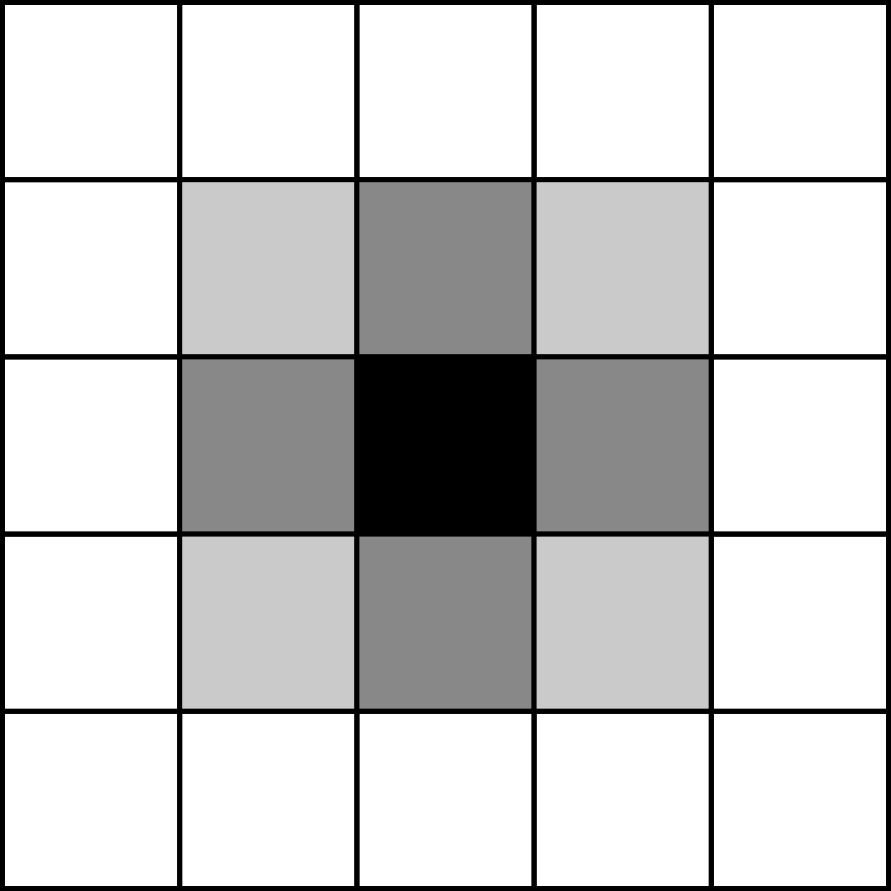
\includegraphics[width=0.3\linewidth]{resources/neighbourhood.png}
    \end{center}
    \caption{The neighbourhood of the black pixel consists of the grey pixels in
    4-connectedness. In 8-connectedness also the light grey pixels are part of the
    neighbourhood}.
    \label{fig:neighbourhood}
\end{figure}

The zero-crossing algorithm starts by calculating the magnitude of the gradient
using the laplacian function included inside the scikit-image library. To
extract the zero-crossings the program will iterate over the whole array
(excluding the border) and checks a single condition. Given its position $(i, j)$
the algorithm checks if $|\nabla I(i, j))| < 0$ and its neighbours have
non-negative magnitude of the gradient.  If this condition stands, then there is
a zero-crossing at position $(i, j)$. In this case the neighbourhood is
calculated as 4-connectedness. 4-connected means that the neighbourhood of the
pixel consists of the pixels on top, left, bottom, and right of the pixel as is
shown in Figure \ref{fig:neighbourhood}.

\subsection{Markers for watershed algorithm}
Extraction of the markers for the watershed function is not as trivial as it
might seem. The algorithm tries to solve this issue, by taking the result of the
zero-crossing algorithm and fills in the individual cells. To accomplish this
a flood filling algorithm is used.

\begin{figure}
    \begin{center}
        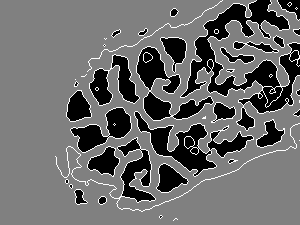
\includegraphics[width=\linewidth]{resources/flood_fill.png}
    \end{center}
    \caption{segmenting cells after zero-crossing algorithm.}
    \label{fig:flood_fill}
\end{figure}

We obtain a binary image from the zero-crossing algorithm. Right now there are
only two values, $0$ stands for background while $255$ stands for the found
edges. We assume that the user usually puts the whole specimen into the view;
therefore we assume that the borders of image belong to the background. Thus,
the program iterates over the borders of the image. If at the currently look at
position there is a background pixel, a flood fill is ran from there with a new
value of $128$. After all the iterations are done, we are left with a grayscale
image with three possible values, $0$ represents the original background, $128$
represents all the space, which was filled during the last step, and $256$
indicates the original edges. The program has managed to separate the insides of
the cells and the background as can be seen on the middle image in Figure
\ref{fig:flood_fill}. Now we can use the newly acquired labelling to create a
segmentation of cells as is seen in the last picture in the previously mentioned
Figure.

\begin{figure}
    \begin{center}
        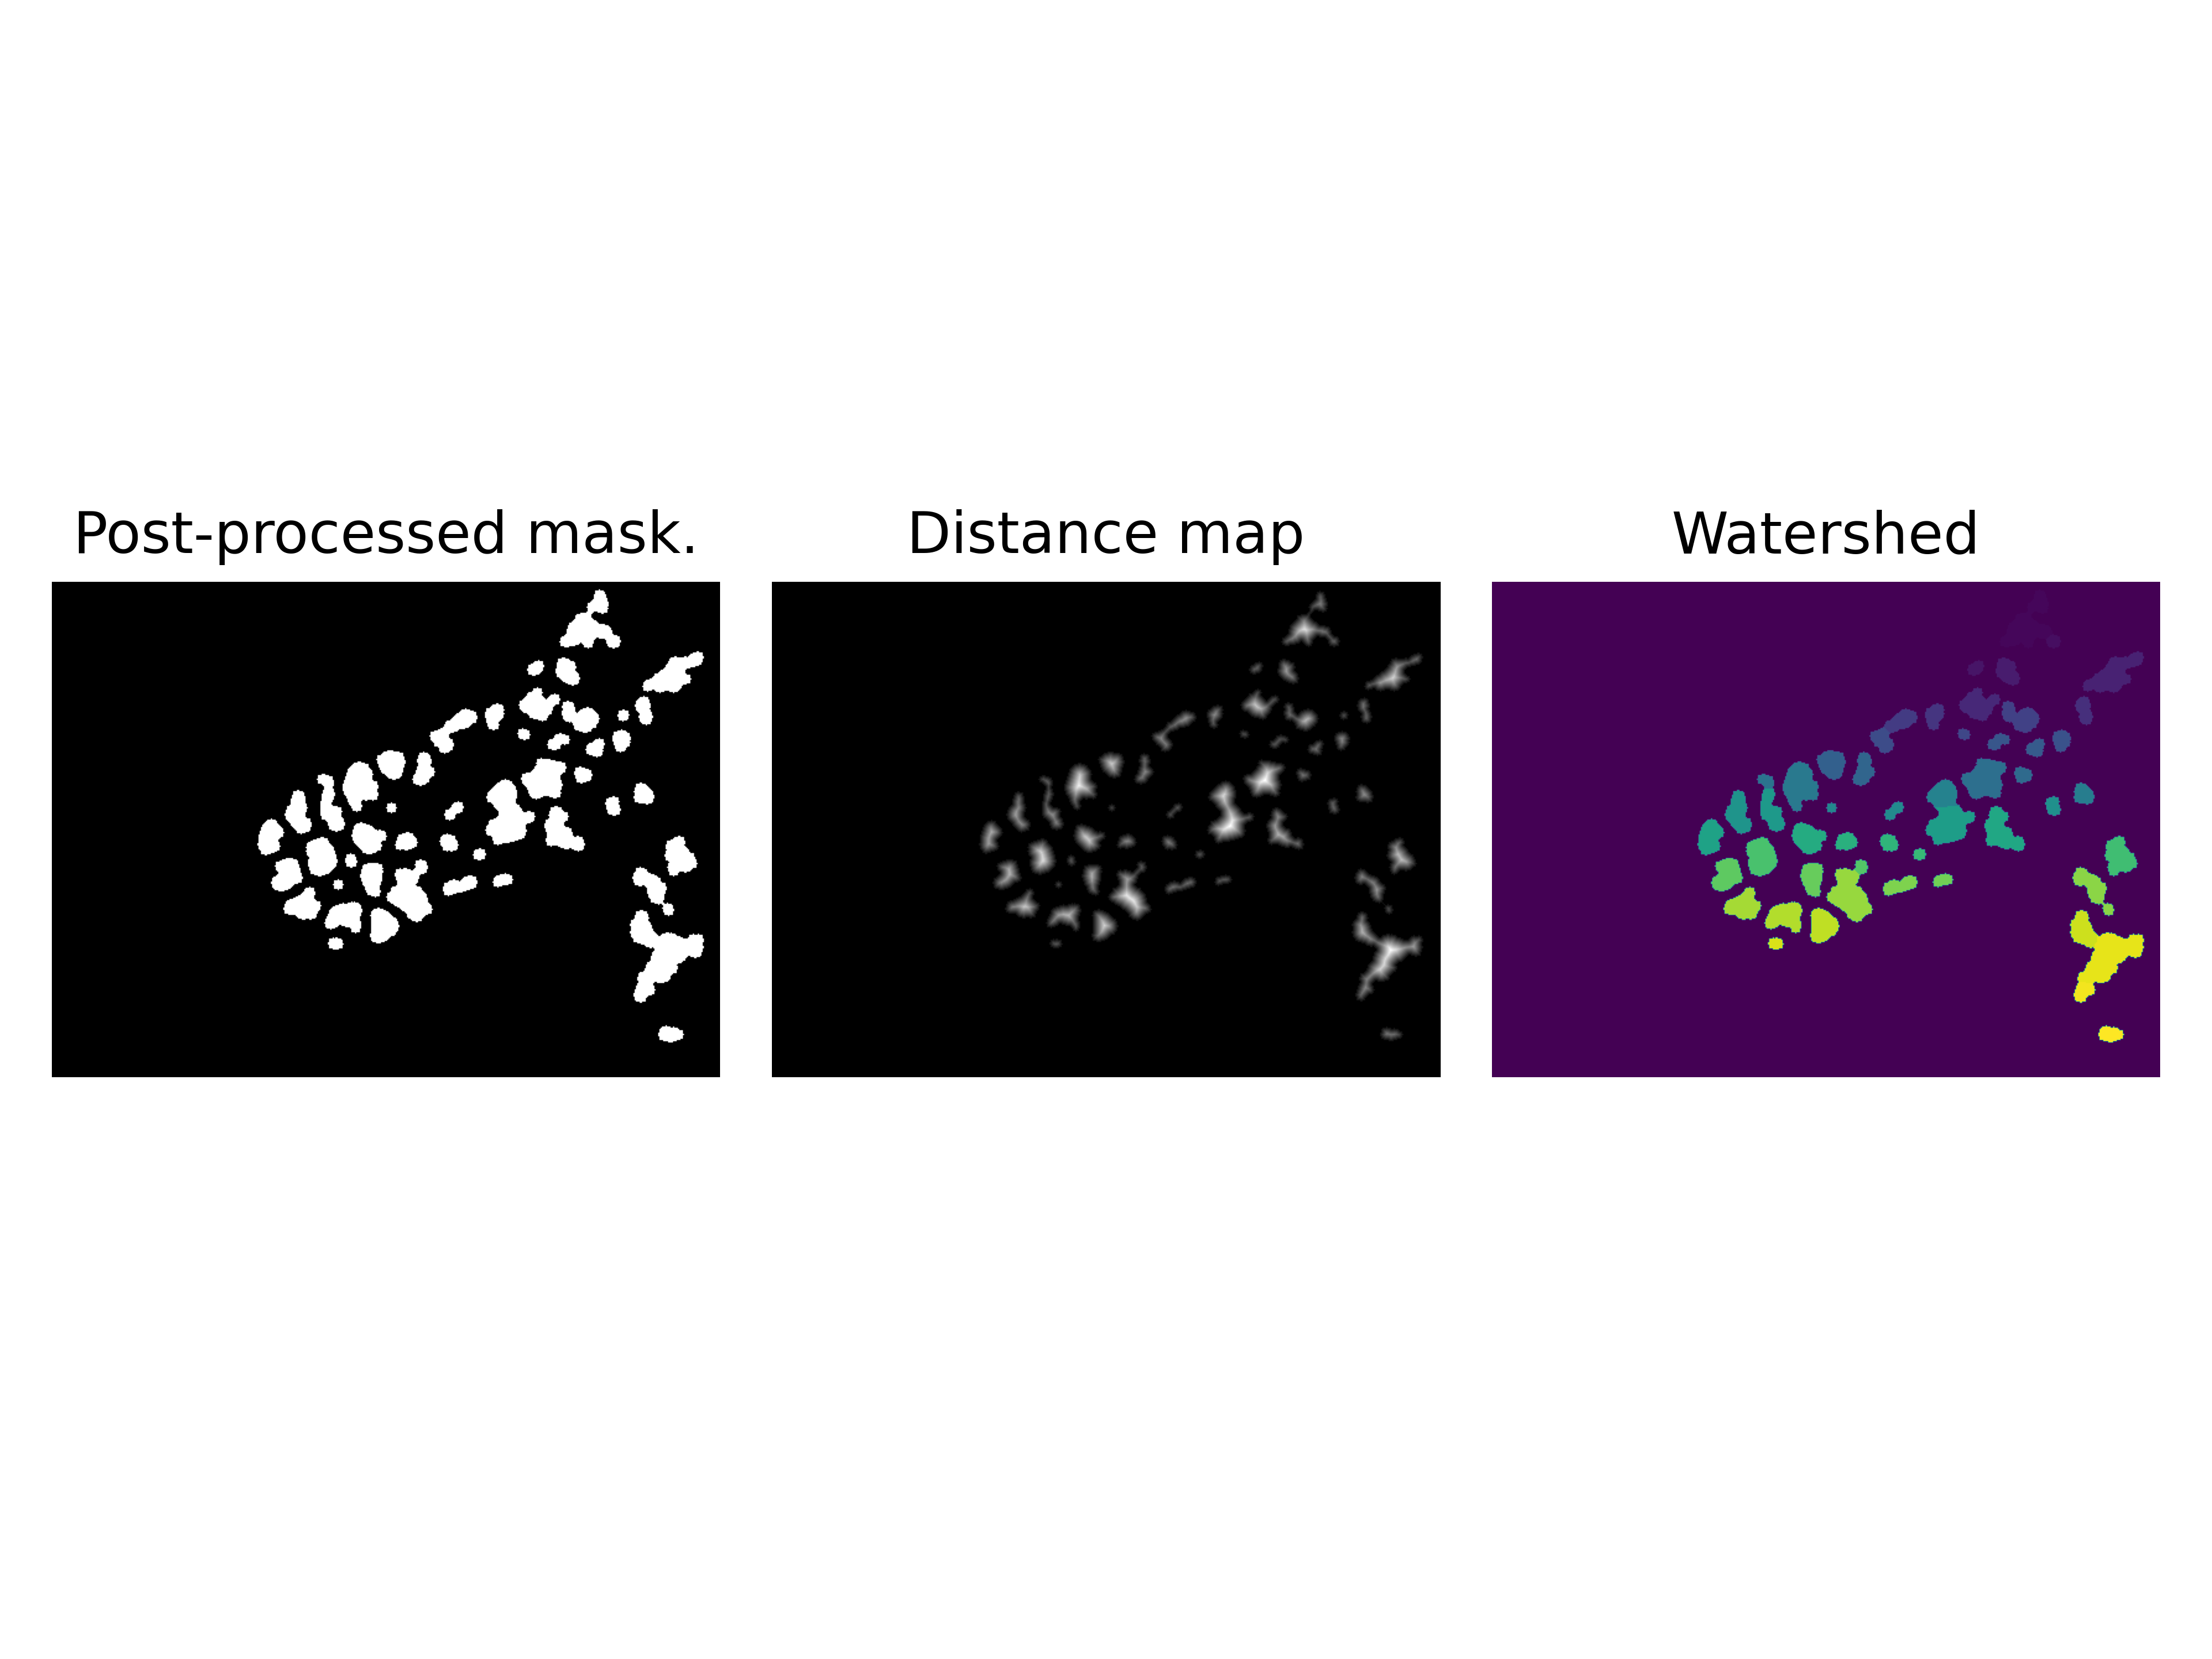
\includegraphics[width=\linewidth]{resources/distance_map.png}
    \end{center}
    \caption{Distance map.}
    \label{fig:distance_map}
\end{figure}

Before this can be applied in the next steps, some of the smaller cells clearly
outside of the specimen has to be removed. These are caused by the imperfections
in the denoising parts. Even after the maximum projection and the cell mask are
applied, in many cases, some residual noise can create small fake cells. To
remove them a morphological opening is performed, leading to the left image in
Figure \ref{fig:distance_map}.

Now that the cells were segmented, the distance map is calculated. This is shown
as the right image in Figure \ref{fig:distance_map}. The distance map was
calculating using the SciPy library and it uses Euclidean distance.

Next, to extract the markers the peaks inside the distance map were found using
the \texttt{peak\_local\_max} from the scikit-image library. The benefit of
this function is that the user can provide a minimum distance separating two
markers. Additionally, the function allows the user to specify threshold, that
means that peaks with low intensity will be ignored, further improving the
labelling.

Finally, the watershed algorithm is run on the distance map, with the results
visualised in the 3rd image in Figure \ref{fig:distance_map}.

\subsection{Maximum projection} To calculate the maximum projection of the data,
the program calculates the Gaussian pyramid using the \texttt{pyramid\_gaussian}
function from the scikit-image library. After this, the images are resized to
the previous size using the \texttt{resize} function from scikit-image.

Projecting is done by iterating over the every position in 2D and finding the
maximum at the given position from all the given layers. The result are shown in
Figure \textbf{TODO}.

That concludes all the non-trivial parts of the program, the rest were a direct
application of functions in the aforementioned libraries.

\subsection{Gradient threshold}
\textbf{TODO: I dont know if this should be in here.}

\chapter{Evaluation}
\label{chp:evaluation}
This chapter deals with the evaluation of the results, common problems, and the
performance of the pipeline. Two metric will be defined and analysed on part of
the data set.

\section{Scoring of the algorithm}

We created two key measures to evaluate the results. To test how many cells were
detected, we devised a detection quality score using F1 measure, and to test the
quality of the segmentation, a test based on the Jaccard score was created.
\begin{figure}
    \begin{center}
        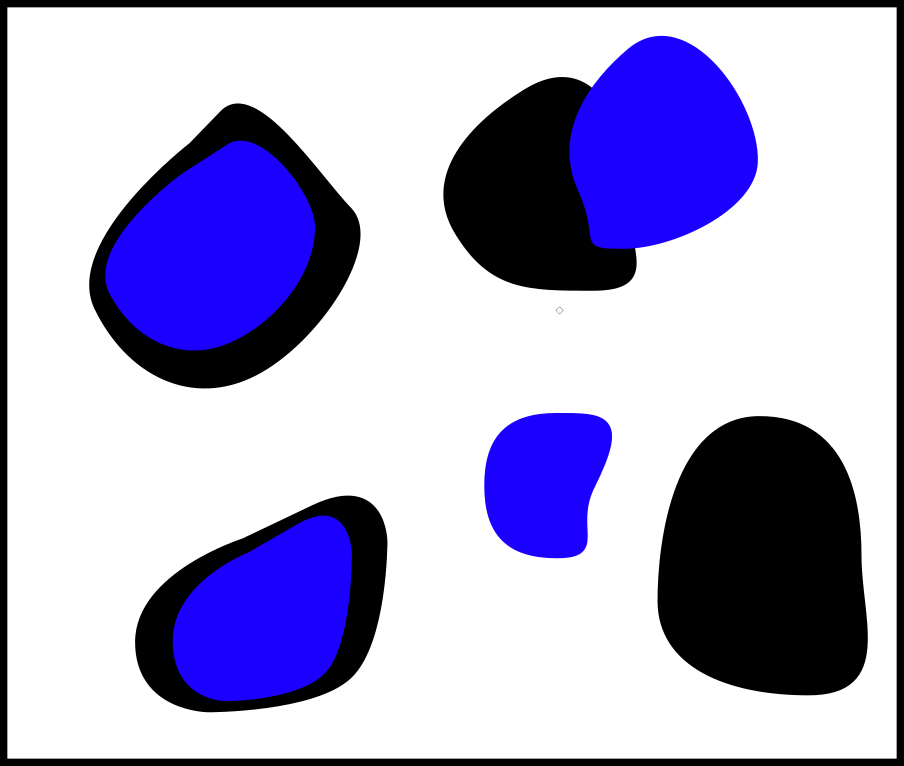
\includegraphics{resources/inkscape/evaluation.png}
    \end{center}
    \caption{Simplified model of cells. Blue cells were predicted by the program
    while the black ones are cells found by the expert.}
    \label{fig:evaluation_basic}
\end{figure}
To talk about the scoring, we need to define a way how to pair the real cell
with the predicted segmentation. A simplified model of the problem is in Figure
\ref{fig:evaluation_basic}. The blue cells in the figure are the program's
prediction, while the black cells are real, created by an expert. As can be seen
the prediction on left are quite good as they cover the majority of the real
cell, while in the top right part, the program did not manage to properly
segment the cell, and in the bottom right the program missed completely,
creating a new imaginary cell, which was not found by the expert.

To take the analysis further, we need a way how to pair the relevant predictions
with the real segmentations. In the simplified diagram I only used two colours
to denote the predicted and real cells; however, in the real segmentation, each
cell has a unique label. To complicate things further, the similar cells do not
have to have the same label in the predicted and real segmentation.

Solving this problem was done using a simple metric based on set operations.
Looking at each cell as a set of its pixels, we can talk about the intersection
of two cells. To illustrate, take a look at the cells in the top left corner of
the aforementioned figure. If we consider the two cells are sets of their
pixels, their intersection is equal to the whole blue set, and the union is
equal to the black set.

In general, picking a single real cell and one predicted cell, we can construct
two sets containing their pixels. Set containing the pixels of the real cell is
denoted as $R_i$, while the second set containing the pixels of the predicted
cell is denoted as $P_i$. If the intersection is large enough, these are two
cells are considered to be a pair. These pairs are later used in the quality
metrics. In full, the condition is
$$|R_i \cap S_i| > \alpha * |R_i| \Leftrightarrow R_i \text{ and } S_i \text{ form a pair}$$
for some threshold $\alpha$. By default this threshold is set to 0.5, ensuring
that every $R_i$ can have just one pairing member $S_i$. Towards the end of this
chapter, this threshold is changed, to analyse how does the scoring change based
in this threshold.

\subsection{Segmentation quality}
\begin{figure}
    \begin{center}
        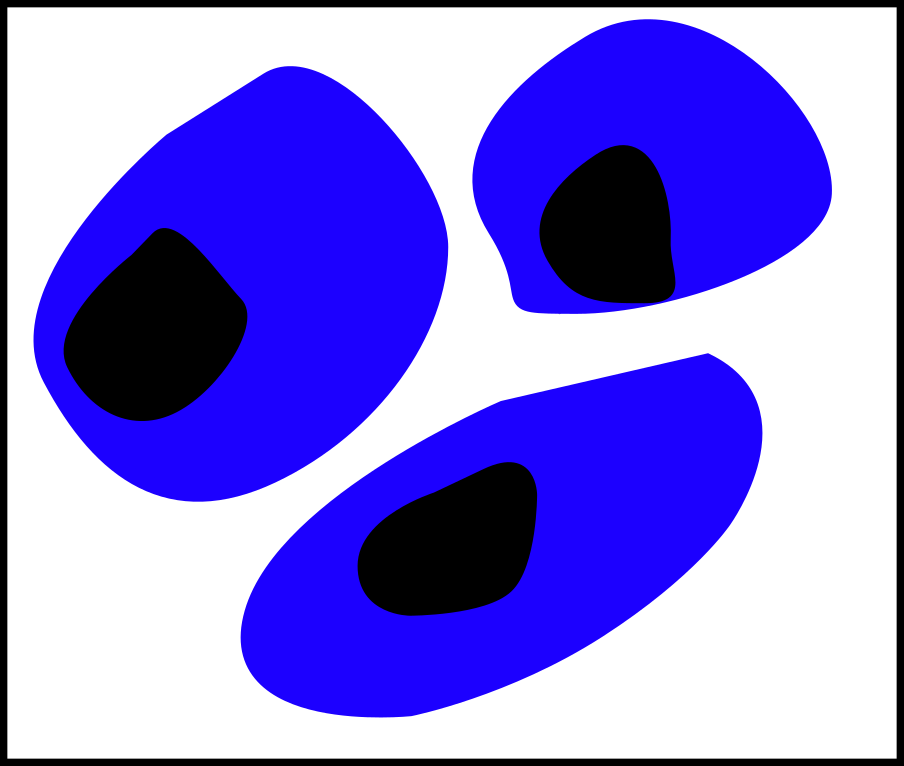
\includegraphics{resources/inkscape/evaluation_imprecise_segmentation.png}
    \end{center}
    \caption{Segmentation where the program labelled a lot of extra area.}
    \label{fig:evaluation_imprecise}
\end{figure}
First metric tries to evaluate how well does the predicted segmentation overlap
with the expert's segmentation. Just checking the size of the intersection is
not good enough, as if the program just created large blobs as in Figure
\ref{fig:evaluation_imprecise}, they would technically contain the whole cell;
however, such a result is not satisfactory, because the segmentation contains a
lot of area around the cell.

To take this into account, the segmentation quality is evaluated using the
Jaccard index. Jaccard index of two sets $A$ and $B$ is defined
as\cite{2020eelbode}:
$$J(A, B) = \frac{|A \cap B|}{|A \cup B|}$$
The range of the Jaccard index is from 0 to 1 (included). If the two sets are
identical, then the Jaccard index is equal to 1, while if the two sets do not
have any identical elements, the index is equal to 0.

The benefit of this index is that unlike plain intersection, the size of the two
sets are taken into account; therefore, the improper segmentation in
\ref{fig:evaluation_imprecise} would cause the index to be quite low, since the
denominator would be much larger than the numerator.

In the final evaluation, after the pairing, the Jaccard index of each pair of
cells will be calculated and averaged, leading to a metric of how well did the
program segment the data. Sometimes, the program's segmentation completely
misses few cells the found areas fail the pairing condition, so some cells found
by the expert do not belong to any pair. We decided to score these cells as
having 0 Jaccard index. If these cases are counted in average, the average is
denoted using the symbol $\overline{J}$. If these cases are ignored in the
average, the symbol $\overline{J_S}$ is used.

\subsection{Detection quality}
\begin{figure}
    \begin{center}
        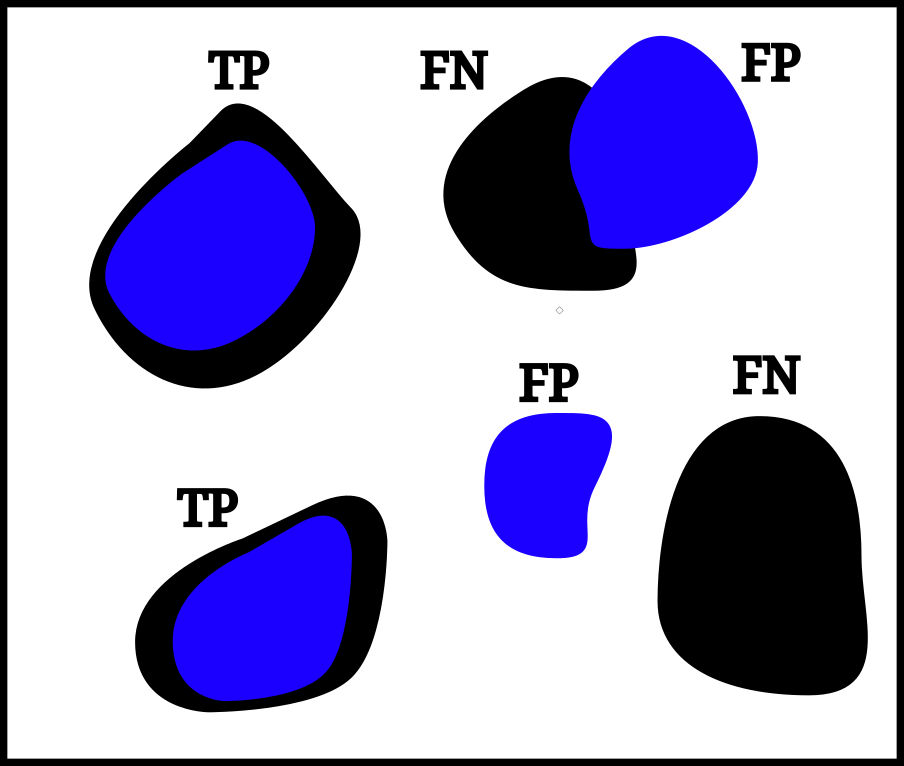
\includegraphics{resources/inkscape/evaluation_with_TP.png}
    \end{center}
    \caption{A simplified model of the cells, including which are considered to
    be true positives, false negatives, and false positives.}
    \label{fig:evaluation_with_TP}
\end{figure}

%todo: mozno citacia na confusion matrix
Apart from the quality of the segmentation, a useful metric is how many cells
the program was able to find compared to how many were found by the expert. The
concept of pairs from the previous section is also used here to pair up the
predictions with the real cells. If a pair is found, then it is considered as a
true positive. If a cell found by an expert does not have a partner, then it is
considered to be a false negative, and if a cell found by the program does have
a corresponding cell found by an expert, it is considered to be a false
positive. In Figure \ref{fig:evaluation_with_TP} this idea is visualised.
%todo: missing TN

Now that the notion of true positives, false positives, and false negatives have
been mapped to our results, a standard F1 score can be applied. It is defined as
the harmonic mean between recall and precision \cite{sklearn-f1score}, formally:
$$\text{recall} = \frac{\text{TP}}{\text{TP} + \text{FN}}$$
$$\text{precision} = \frac{\text{TP}}{\text{TP} + \text{FP}}$$
$$F_1 = \frac{2 * \text{recall} * \text{precision}}{\text{recall} +
\text{precision}}$$
Generally speaking, recall is a useful measure to see how many of the predicted
cells are actual cells. If our system has low recall, that means that a
significant number of cells found by the expert were missed by our program. On
the hand, precision talks about how many of the program's predictions are actual
cells. Then the F1 score is just a useful overall measure, taking into account
undersegmenting and oversegmenting in our data.

\subsection{Results}
When evaluating the dataset, I took each image and gave myself around 2--7
minutes to find the best segmentation. First I visually inspected the results,
and tried to tweak the parameters to fix some of the common issues. After I was
satisfied with the results I tried to tweak the parameters again, this time
evaluating the $\overline{J_s}$ score. After that, I recorded the results, and
proceeded to the next image.

The final results are recorded in Table \ref{tab:scores}. Every row begins
with the filename and provides various scores I was able to achieve with the
program. As can be seen from the table, certain images got better results than
the other. 

In general, the program has higher recall than precision, meaning that the
program finds the majority of the cells marked by the expert; however, it also
find many false positives. Those are cells, that the program predicted, but were
not found by the expert.

Looking at the $\overline{J_S}$ scores, it is clear, that if the program finds a
real cell, it segments it reasonably well. To further investigate this, I listed
the Jaccard scored for found pairs in the evaluation of the file
\texttt{t004-roi-10} in Table \ref{tab:scores_roi10}. In this particular case,
all of them were above 0.5, but in some cases the segmentation produces Jaccard
scores bellow 0.5 (for example, when two real cells are marked as a single large
blob).

\begin{table}
    \begin{tabular}{|| c|c|c|c|c|c ||}
        \toprule
        File name & $\overline{J}$ & $\overline{J_S}$ & $F\_1$ & Precision & Recall \\
        \midrule
        t002-roi-1&0.35&0.65&0.462&0.40&0.545\\
        t002-roi-2&0.34&0.54&0.53&0.46&0.63\\
        t004-roi-4&0.47&0.62&0.53&0.41&0.77\\
        t004-roi-4&0.68&0.68&0.39&0.24&1.00\\
        t004-roi-6&0.38&0.61&0.62&0.60&0.63\\
        t004-roi-10&0.45&0.72&0.68&0.75&0.63\\
        t004-roi-11&0.45&0.63&0.59&0.50&0.72\\
        t006-roi-2&0.39&0.59&0.53&0.44&0.67\\
        t006-roi-5&0.29&0.63&0.42&0.39&0.46\\
        \bottomrule
    \end{tabular}
    \caption{TODO}
    \label{tab:scores}
\end{table}

\begin{table}
    \begin{tabular}{||c||}
        \toprule
        $J_i$\\
        \midrule
        0.913\\
        0.783\\
        0.836\\
        0.727\\
        0.587\\
        0.867\\
        0.810\\
        0.670\\
        0.564\\
        0.693\\
        0.750\\
        0.535\\
        0.791\\
        0.795\\
        \bottomrule
    \end{tabular}
    \caption{TODO}
    \label{tab:scores_roi10}
\end{table}

\subsection{Changing the threshold}

\textbf{TODO: Pick a single image and try different thresholds. Plot the F1 and
Jaccard scores.}

\subsection{Performance}

\textbf{TODO:} Try running the whole program on the whole dataset multiple
times. Create the average and st. deviation. Also monitor the RAM usage.

\section{Common problems}

\textbf{TODO: obrazky plus popis}
\begin{itemize}
    \item Obrazky niekedy treba orezat, aby sa vyplnili stredy.
    \item Nejasne okraje medzi bunkami: prelievanie.
    \item Nejasny okraj medzi vnutrami okraj. buniek a pozadim robia blbosti
\end{itemize}

\chapter{Conclusion}

\end{document}
